% Esta es la Plantilla UNAL en LaTeX
\documentclass[11pt,spanish,fleqn,openany,twoside,letterpaper]{book}

%Muestra los márgenes del documento para evitar Warnings
%Para activar la siguiente línea quite el simbolo % 
%\usepackage[showframe]{geometry}

%Formato de fuentes bibliográficas
%Use el estilo bibliográfico que sea pertinente según el área de estudio APA, IEEE, etc

%Usando el paquete BibLaTeX
%Cita normal con \cite[página]{} y cita con paréntesis \parencite[página]{}

% Configuración de BibLaTeX (se usa una sola vez más abajo)

% Cambiar el idioma de las referencias bibliográficas a español
%\DefineBibliographyStrings{spanish}{%
%  andothers = {et\addabbrvspace al\adddot},
%  andmore = {et\addabbrvspace al\adddot},
%}

% Personalizar el formato de las citas y la bibliografía
%\DeclareNameAlias{sortname}{family-given}
%\DeclareDelimFormat{multinamedelim}{\addcomma\space}
%\DeclareDelimFormat{finalnamedelim}{\addcomma\space\&\space}
%\DeclareFieldFormat{titlecase}{\MakeSentenceCase*{#1}}
%\DeclareFieldFormat[article,inbook,incollection,inproceedings,patent,thesis,unpublished]{title}{\titlecase{#1}}
%\DeclareFieldFormat{journaltitlecase}{\titlecase{#1}}
%\DeclareFieldFormat{pages}{#1}
%\DeclareFieldFormat{volume}{\mkbibbold{#1}}
%\renewbibmacro{in:}{}
%\AtEveryBibitem{\clearfield{month}}

% Bibliografía: usar biblatex + biber (más moderno) OR mantener natbib/bibtex
% Si quieres usar biber, activa las siguientes líneas. Si prefieres bibtex/natbib,
% mantén las líneas comentadas y usa `bibtex` en lugar de `biber`.
\usepackage[utf8]{inputenc}
\usepackage{csquotes}
\usepackage{iftex}


%Idioma del documento
%Use main para el idioma principal del documento
\usepackage[main=spanish,english,german,french,portuguese]{babel}
\usepackage{textgreek}
% Carácteres especiales
\usepackage[T1]{fontenc}
\usepackage{fontspec}


% Evita ligadura li & fl
% Nota: DisableLigatures no funciona con XeLaTeX, solo con pdfLaTeX
\usepackage{microtype}
%\DisableLigatures{encoding = *, family = *}

% Otros paquetes de tablas y colores avanzados
\usepackage{amsmath,graphicx,rotating,float,multirow}
\usepackage{longtable}
\setlength{\LTcapwidth}{6in}
\usepackage{epsfig,epic,eepic,threeparttable,amscd,here,lscape,tabularx,subfigure}
\usepackage{tabu,array}
\usepackage[rgb]{xcolor}
\usepackage{colortbl}

% Permite ver y configurar los parámetros de la página
\usepackage{layout}
%Hyperref permite ver las secciones del texto
\usepackage[hidelinks,pdfpagelayout=SinglePage]{hyperref}

%Permite incluir código de cualquier lenguaje dentro del texto del documento
\usepackage{minted}
\usepackage{fancyvrb}
\newenvironment{myverbatim}{\Verbatim}{\endVerbatim}

%Genera los comandos de la página de autoría
\newcommand{\studentname}{}
\newcommand{\submissiondate}{}
\newcommand{\academictitle}{}
\newcommand{\resgroupone}{}
\newcommand{\resgrouptwo}{}
\newcommand{\researchtopic}{}
\newcommand{\thesisname}{}
\newcommand{\thesisnameeng}{}
\newcommand{\thesisnamelang}{} %Usar solo si se requiere
\newcommand{\director}{}
\newcommand{\directortitle}{}
\newcommand{\codirector}{} %Usar solo si se requiere
\newcommand{\codirectortitle}{} %Usar solo si se requiere
\newcommand{\issuedate}{}
\newcommand{\palabrasclave}{}
\newcommand{\keywords}{}
\newcommand{\schlusselworter}{}
\newcommand{\palavraschave}{}
\newcommand{\sede}{}
\newcommand{\department}{}
\newcommand{\departmenttwo}{} %Usar solo si se requiere
\newcommand{\faculty}{}
\newcommand{\university}{Universidad Nacional de Colombia}
%Información de la tesis
%Diligenciar aquí los datos para su carga automática donde se requiera en el documento
%En el caso de tesis o trabajos finales, verificar que el título coincida con el aprobado por la Facultad
\renewcommand{\thesisname}{Diseño de tareas matemáticas con IA generativa para el desarrollo del pensamiento trigonométrico en educación media}
\renewcommand{\issuedate}{2025}
\renewcommand{\directortitle}{Profesor Asociado}
\renewcommand{\codirector}{Dra.~Marisol Santacruz Rodríguez \\
Dr. Luis Octavio Gonzalez Salcedo}}
%\renewcommand{\codirectortitle}{Indicar si es Profesor Titular/Asociado}
%\renewcommand{\academictitle}{Magíster (M, MSc) o Doctor (PhD) - Modalidad }
\renewcommand{\resgroupone}{Grupo A (Sigla Grupo Investigación 01) }
\renewcommand{\resgrouptwo}{Grupo B (Sigla Grupo Investigación 02) }
\renewcommand{\researchtopic}{Línea}
\renewcommand{\sede}{Sede Palmira} 
\renewcommand{\department}{}
\renewcommand{\departmenttwo}{Departamento 2} %Usar solo si es necesario
\renewcommand{\faculty}{Facultad de Ingeniería y Administración}

%Palabras clave del documento - Tener presente los Theasurus https://www.thesaurus.com/
%Disponible en 3 idiomas aunque se puede extender a francés o otro idioma
\renewcommand{\palabrasclave}{inteligencia artificial generativa; pensamiento trigonométrico; tareas matemáticas; software educativo; educación media}
\renewcommand{\keywords}{generative artificial intelligence; trigonometric thinking; mathematical tasks; educational software; secondary education}
%\renewcommand{\schlusselworter}{}
%\renewcommand{\palavraschave}{}

% Estilo de los encabezados y pies de página
\usepackage{fancyhdr}
\fancyhf{}%
\pagestyle{fancyplain}
% Márgenes estilo UNAL Word: Superior 3cm, Inferior 3cm, Izq 4cm, Der 2cm
% Con twoside: inner (encuadernación) 4cm, outer 2cm, bindingoffset adicional
\usepackage[top=3cm, bottom=3cm, inner=4cm, outer=2cm, bindingoffset=0cm]{geometry}
\fancypagestyle{plain}{
\fancyhf{}
\fancyhead[LE]{}
\fancyhead[RO]{}
\fancyfoot[C]{\thepage}
\renewcommand{\headrulewidth}{0pt}
}
\pagestyle{fancy}
\fancyhf{}%
\fancyhead[LE]{\thepage}
\fancyhead[RO]{\thepage}
\fancyfoot[C]{}
\renewcommand{\headrulewidth}{0pt}

\usepackage{titlesec}
% Permite personalizar los títulos de sección y de capítulos
% hang lo deja en el mismo renglón, display lo despliega
% Elimina el "Capitulo" y deja solo el número
% Formato de títulos estilo Word UNAL
\titleformat{\chapter}[display]
  {\normalfont\bfseries\filcenter}{\Large CAPÍTULO \thechapter}{10pt}{\Large\MakeUppercase}
\titleformat{\section}
  {\normalfont\large\bfseries}{\thesection}{1em}{}
\titleformat{\subsection}
  {\normalfont\normalsize\bfseries}{\thesubsection}{1em}{}
\titleformat{\subsubsection}
  {\normalfont\normalsize\bfseries}{\thesubsubsection}{1em}{}
\titleformat{\paragraph}[runin]
  {\normalfont\normalsize\bfseries}{}{}{}

% Espaciado antes y después de títulos
\titlespacing*{\chapter}{0pt}{0pt}{20pt}
\titlespacing*{\section}{0pt}{12pt}{6pt}
\titlespacing*{\subsection}{0pt}{12pt}{6pt}
\titlespacing*{\subsubsection}{0pt}{12pt}{6pt}

%Coloca anexo o apéndice en la Tabla de contenido
\usepackage[toc,page]{appendix}

% Configuración de las páginas estilo Word
% Espaciado entre párrafos
\setlength{\parskip}{6pt}
% Sangría de primera línea
\setlength{\parindent}{1.25cm}
\renewcommand{\theequation}{\thechapter-\arabic{equation}}
\renewcommand{\thefigure}{\textbf{\thechapter-\arabic{figure}}}
\renewcommand{\thetable}{\textbf{\thechapter-\arabic{table}}}

%Ajusta el espacio entre la etiqueta de figuras y tablas y su título en la lista de figuras y en la de tablas 
\usepackage{titletoc} 
\titlecontents{figure}[0em]{}{\thecontentslabel\hspace{1em}}{}{\titlerule*[1pc]{.}\contentspage}
\titlecontents{table}[0em]{}{\thecontentslabel\hspace{1em}}{}{\titlerule*[1pc]{.}\contentspage}

%Define la distancia de la primera linea de un parrafo a la margen
% (configurado arriba con \parindent)

%Espacio entre lineas - 1.5 como en Word
\renewcommand{\baselinestretch}{1.5}

%Permite personalizar el ajuste vertical mediante cajas
\usepackage{adjustbox}

%Para rotar texto, objetos, tablas y páginas.
\usepackage{rotating}

%Permite incluir mecanismos y reacciones químicas
\usepackage{tikz}
\usepackage{pgfplots}
\pgfplotsset{compat=1.18}
\usepackage{chemformula}
\usepackage{chemfig}

\usetikzlibrary{calc,arrows.meta,angles,quotes}% per right to e left to
\tikzset{
myedge/.style={->, -{Latex[#1]}}
}

%Fuente de la presentación Ancizar Sans UNAL
%Para usar este compilado en Overleaf se debe usar el compilador XeLaTeX o LuaLaTeX!!
%Menu -> Compiler -> XeLaTeX o LuaLaTeX
%La siguiente línea debe comentarse si desea compilar con pdfLaTeX
%\RequireXeTeX

% Definición de la fuente Ancizar Sans
\newif\ifxetexorluatex
\ifXeTeX
  \xetexorluatextrue
\fi
\ifLuaTeX
  \xetexorluatextrue
\fi

\ifxetexorluatex
  % Usar Arial si existe; en caso contrario, usar Liberation Sans.
  \IfFontExistsTF{Arial}
    {\setmainfont{Arial}[Ligatures=TeX,Scale=1.0]}
    {\setmainfont{Liberation Sans}[Ligatures=TeX,Scale=1.0]}
  \setsansfont{Liberation Sans}
\else
  % Si se compila con pdfLaTeX
  \usepackage[T1]{fontenc}
  \usepackage{helvet}
  \renewcommand{\familydefault}{\sfdefault}
\fi
% Metadatos del documento
\AtBeginDocument{%
	\hypersetup{
		pdfborder={0 0 0},
		pdfauthor={\studentname},
		pdfsubject={\thesisname}, 
		pdfcreator={\studentname},
		pdfproducer={\studentname},
	}
}

%Carga el simbolo de grado y el de Angstrom
\newcommand{\angstrom}{\textup{\AA}}
\newcommand{\grad}{\(^{\circ}\)}

%bibliografia

\usepackage[backend=biber,style=apa,maxcitenames=2,maxbibnames=99,giveninits=true,uniquename=false]{biblatex}
\addbibresource{bibliografias/antecedentes.bib}
\addbibresource{bibliografias/antecedentes/antecedentes.bib}
\addbibresource{bibliografias/antecedentes/ia-en-eduacion-matematica/ia-en-educacion-matematica.bib}
\addbibresource{bibliografias/antecedentes/ia-en-enseñanza-de-la-trigonometria/ia-en-enseñanza-de-trigonometria.bib}
\addbibresource{bibliografias/antecedentes/dificultades-percistentes-en-trigonometria-escolar/dificultades-persistentes-en-trigonometria-escolar.bib}
\addbibresource{bibliografias/Planteamiento_del_problema.bib}
\addbibresource{bibliografias/justificacion/jusitificacion.bib}
\addbibresource{bibliografias/justificacion/justificacion_pedagogica_didactica/justificacion_pedagogica_didactica.bib}
\addbibresource{bibliografias/justificacion/justificacion_social_tecnologica/justificacion_social_tecnologica.bib}
\addbibresource{bibliografias/marcos_teorico/marco_conceptual/marco_conceptual.bib}
\addbibresource{bibliografias/marcos_teorico/identificacion_del_marco_teorico/identificacion_del_marco_teorico.bib}
\addbibresource{bibliografias/antecedentes/Nivel_1.bib}
\addbibresource{bibliografias/antecedentes/Nivel_2.bib}
\addbibresource{bibliografias/antecedentes/Nivel_3.bib}


%Inicio del documento, no olvide la etiqueta de cierre al final \end{document}
\begin{document}

%Nombres y formatos de títulos, tablas y figuras
\renewcommand{\listfigurename}{Lista de figuras}
\renewcommand{\listtablename}{Lista de tablas}
\renewcommand{\contentsname}{Contenido}
\renewcommand{\chaptername}{Capítulo}
\renewcommand{\tablename}{\scriptsize \centering \textbf{Tabla}}
\renewcommand{\figurename}{\scriptsize \centering \textbf{Figura}}
\renewcommand{\appendixname}{Anexo}

%Cambia el nombre de la sección de referencias
\renewcommand{\bibname}{Referencias Bibliográficas}

%Páginas de Presentación del documento - Portada estilo UNAL
{\newpage
\thispagestyle{empty}
\begin{center}

\vspace*{1cm}

\begin{figure}[h]
\centering

\epsfig{file=imagenes/00Figuras/00f00EscudoUN2016,scale=0.7}%
\end{figure}

\vspace{1.5cm}

\textbf{\LARGE \thesisname}

\vspace{0.5cm}

\textbf{\Large \studentname}

\vspace{0.5cm}

Directores de tesis:

\vspace{0.5cm}

{\director}\\[0.3cm]
{\codirector}

\vspace{\fill}

{\Large \university}\\[0.3cm]
{\large \faculty}\\[0.2cm]
{\normalsize Maestría en Enseñanza de las Ciencias Exactas y Naturales}\\[0.3cm]
{\normalsize \sede, Colombia}\\[0.2cm]
{\normalsize \issuedate}

\end{center}

% Dedicatorias - COMENTADA (descomentar si se desea usar)
%\newpage
%\thispagestyle{empty}
%\begin{flushright}
%\begin{minipage}{12.5cm}
%\noindent
%\vspace{10em}
%
%%Modificar la cita que se quiere agregar
%%{\Large Cita 01.}
%
%%\vspace{3em}
%
%%Autor
%
%%\textit{Fuente}
%
%\vspace{10em}
%
%%Para anular la adición de una segunda cita anule las siguientes lineas desde acá mediante comentario (%)
%%{\Large \textit{Wenn du es nicht einfach erkl\"{a}ren kannst, hast du es nicht genug verstanden} --- Si no eres capaz de explicar algo claramente, es que aún no lo has entendido lo suficiente.}
%
%%\vspace{3em}
%
%%Albert Einstein
%%Hasta acá!
%\end{minipage}
%\end{flushright} 

% Declaracíon de originalidad del texto y del contenido
% No modificar, se hace automáticamente con los comandos ya definidos
%\newpage
%\chapter*{Declaración}
%\par Me permito afirmar que he realizado ésta tesis de manera autónoma y con la única ayuda de los medios permitidos y no diferentes a los mencionados el presente texto. Todos los pasajes que se han tomado de manera textual o figurativa de textos publicados y no publicados, los he reconocido en el presente trabajo. Ninguna parte del presente trabajo se ha empleado en ningún otro tipo de tesis. 

%\vspace{1em}

%{\sede}, {\submissiondate}

%\vspace{6em}

%\rule{6cm}{0.5pt}\\
%{\studentname}
%}

%Páginas preámbulo, listado de figuras, tablas y tabla de contenido
{\pagestyle{plain} \pagenumbering{roman}
\setlength{\parskip}{1mm}
%\input{capitulos/01_preambulo/agradecimientos/00Agradecimientos}
% Comentar las dos lineas de abajo con % en caso que no se requieran abreviaturas y resumen en el trabajo
%\input{capitulos/01_preambulo/abreviaturas_simbolos/00Abreviaturas}
%\input{capitulos/01_preambulo/resumen/00ResumenAbstract}
% Dejar esta parte así para que genere correctamente la página de la tabla de contenido
\addcontentsline{toc}{chapter}{Contenido}
\tableofcontents
\clearpage
\addcontentsline{toc}{chapter}{Lista de figuras}
\listoffigures
\clearpage
\addcontentsline{toc}{chapter}{Lista de tablas}
\listoftables

}

{\pagenumbering{arabic}
\setlength{\parskip}{\baselineskip}
%Incluir secciones del documento de aqui en adelante
%Use \include para incluir desde una página nueva e \input para incluir sin salto de página
%\chapter*{\sffamily Introducción}

\addcontentsline{toc}{chapter}{\sffamily Introducción}
\markboth{\sffamily Introducción}{}
\clearpage
\newpage
 % Anular esta linea con comentario de ser necesario
\chapter{Planteamiento del Problema}

% Este archivo fuente queda sincronizado con la versión modular del capítulo 3.

La enseñanza de la trigonometría en educación media arrastra una tensión que no logra resolverse. El currículo pide que el estudiantado razone sobre variación, periodicidad y articulación entre registros. En el aula ocurre otra cosa: predominan las fórmulas, los procedimientos y los ejercicios cerrados \parencite{diaz-fernandezEnsenanzaTrigonometria4o2014,rosaEnsenanzaAprendizajeTrigonometria2023}.

La consecuencia es previsible, pero no por eso menos preocupante. Los estudiantes resuelven triángulos rectángulos sin mayor dificultad. Interpretar una gráfica trigonométrica ya es otro asunto. ¿Por qué se rompe ahí la comprensión? Trabajar razones trigonométricas no parece bastar para construir la comprensión funcional que la educación media espera.

La literatura ofrece una pista: estas dificultades se relacionan, en parte, con una enseñanza centrada en el cálculo mecánico y con poco espacio para argumentar \parencite{fiallolealAcercaInvestigacionEducacion2015,delgadoEstrategiaDidacticaPara2023}. Tratar seno, coseno y tangente como funciones reales —y no solo como razones que se calculan— exige tareas distintas. Exige también discusiones más profundas y criterios de evaluación pensados para la comprensión, no solo para el resultado \parencite{torres-corralesResignificacionRazonTrigonometrica2021,escalantegodoyUsoComprensivoRazones2018}.

Hay errores que se repiten con la insistencia de un patrón: confundir razón trigonométrica con función, entender mal la periodicidad, no lograr conectar representación gráfica, expresión algebraica y valor numérico \parencite{zubietaTipificacionErroresDificultades2018,ruedaAproximacionEnsenanzaRazones2012,iriarteDificultadesAprendizajeEcuaciones2025}. En Colombia los reportes de evaluación llevan años documentando estas mismas brechas \parencite{ministeriodeeducacionnacionalmenInformeNacionalSaber2019,icfesProgramaParaEvaluacion2024}.

¿El problema está solo en el estudiante? No parece razonable pensarlo así. El tipo de tarea que se propone también pesa. Cuando una actividad exige explorar, comparar y justificar, se abre espacio para comprender. Cuando se limita a repetir, el aprendizaje se reduce a ejecutar procedimientos \parencite{benitezAprendizajeTrigonometriaMediante2022,delgadoAulaInvertidaRendimiento2024,zambrano-choezEstrategiasParaEnsenanza2025}.

La tecnología, aquí, ofrece algo real. GeoGebra permite ver el cambio en tiempo real y conecta representaciones que de otro modo quedan aisladas \parencite{calderonTecnologiasDigitalesPara2024,agudelocarvajalFortalecimientoProcesoEnsenanza2020}. La IA podría ampliar ese potencial: retroalimentación oportuna, rutas de exploración distintas según quien aprende. Pero solo si la tarea conserva exigencia matemática. Reducida a seguir instrucciones, su aporte al pensamiento trigonométrico es mínimo \parencite{romeroalonsoRolInteligenciaArtificial2024,castillodelpezoUseArtificialIntelligence2024}.

No hay, todavía, evidencia propia de cómo se sostiene ese equilibrio —entre apoyo de la IA y exigencia matemática— en un aula real. Ese vacío motiva este trabajo.

De estas premisas nace la pregunta que define el problema: ¿de qué manera el diseño e implementación de tareas trigonométricas integradas con Inteligencia Artificial puede favorecer el paso desde el cálculo hacia el desarrollo del pensamiento trigonométrico en estudiantes de media?

\section{Declaración de la pregunta del problema de profundización}
El panorama descrito evidencia una problemática estructural en la enseñanza de la trigonometría en educación media colombiana. Por una parte, persisten prácticas centradas en memorización y resolución rutinaria que limitan la comprensión funcional de seno, coseno y tangente \parencite{fiallolealAcercaInvestigacionEducacion2015,delgadoEstrategiaDidacticaPara2023}. Por otra, los estudiantes enfrentan obstáculos conceptuales recurrentes para interpretar la variación periódica, coordinar diferentes representaciones y argumentar matemáticamente sus decisiones \parencite{zubietaTipificacionErroresDificultades2018,ruedaAproximacionEnsenanzaRazones2012}.

Esta situación genera una brecha entre las metas curriculares de educación media y lo que efectivamente ocurre en el aula. Aunque los lineamientos nacionales enfatizan pensamiento variacional, modelación y comprensión de funciones, en la práctica muchos procesos de enseñanza no logran sostener ese tránsito desde la razón trigonométrica hacia el pensamiento trigonométrico \parencite{ministeriodeeducacionnacionalLineamientosCurriculares1998,ministeriodeeducacionnacionalEstandaresBasicos2006,ministeriodeeducacionnacionalDerechosBasicos2016}.

En este contexto, la integración con inteligencia artificial no se asume como un fin en sí mismo ni como sustituto de la actividad matemática escolar. El reto está en diseñar e implementar tareas matemáticas integradas con inteligencia artificial (IA) para apoyar procesos de exploración, argumentación y retroalimentación, manteniendo como foco el desarrollo del pensamiento trigonométrico en estudiantes de educación media \parencite{castillodelpezoUseArtificialIntelligence2024,parrasanchezPersonalizacionRecursosPara2023}.

En consecuencia, la presente investigación plantea la siguiente pregunta problema:

\begin{center}
\textbf{\textit{¿De qué manera el diseño e implementación de tareas matemáticas integradas con inteligencia artificial puede contribuir al desarrollo del pensamiento trigonométrico en estudiantes de educación media?}}
\end{center}

Esta pregunta central se desagrega en las siguientes interrogantes específicas que orientarán el desarrollo investigativo:

\begin{enumerate}
    \item \textbf{¿Qué criterios didácticos debe cumplir una secuencia de tareas matemáticas integrada con IA para promover el desarrollo del pensamiento trigonométrico en educación media?}

    \item \textbf{¿Cómo se integra la IA en el diseño y en la implementación de las tareas sin desplazar el trabajo matemático del estudiante?}

    \item \textbf{¿Qué evidencias de desarrollo del pensamiento trigonométrico emergen en los estudiantes durante la resolución de tareas integradas con IA?}

    \item \textbf{¿Qué dificultades y oportunidades aparecen en el aula al implementar estas tareas en un contexto real de educación media?}
\end{enumerate}

\subsection*{Justificación de la pregunta problema}

La pregunta problema se justifica porque responde a una tensión concreta del aula de matemáticas en educación media: se espera que los estudiantes desarrollen pensamiento trigonométrico, pero en la práctica predominan actividades centradas en procedimientos y respuestas rápidas \parencite{fiallolealAcercaInvestigacionEducacion2015,delgadoEstrategiaDidacticaPara2023}. En ese escenario, la IA puede abrir nuevas posibilidades, pero solo si se integra dentro de tareas bien diseñadas que mantengan el foco en el trabajo matemático del estudiante y no en la automatización de resultados \parencite{castillodelpezoUseArtificialIntelligence2024,parrasanchezPersonalizacionRecursosPara2023}.

Además, la pregunta delimita con claridad el alcance del estudio: educación media, trigonometría escolar y desarrollo del pensamiento trigonométrico. Esta delimitación permite analizar con detalle evidencias de aprendizaje, dificultades y decisiones didácticas en un contexto real de implementación, en lugar de hacer afirmaciones generales sobre tecnología educativa.

En consecuencia, la investigación no busca demostrar que la IA, por sí sola, mejora el aprendizaje. Busca comprender bajo qué condiciones de diseño e implementación una secuencia de tareas matemáticas integradas con IA puede aportar al desarrollo del pensamiento trigonométrico.


\section{Antecedentes}

La revisión de antecedentes que se presenta a continuación se articula en torno a tres ejes de la literatura que fundamentan y delimitan el problema de investigación: el uso de inteligencia artificial en educación matemática, la integración específica de herramientas de IA en la enseñanza de la trigonometría, y las dificultades conceptuales que los estudiantes de educación media exhiben de forma persistente en este campo. La convergencia de estos tres ejes define el espacio específico que el presente estudio busca ocupar, tal como se ilustra en la Figura~\ref{fig:mapa_antecedentes}.

\begin{figure}[H]
\centering
\begin{tikzpicture}[
  fuente/.style={draw=blue!60!black, fill=blue!8, rounded corners=6pt,
                 text width=5.2cm, align=center, inner sep=9pt,
                 font=\small\sffamily},
  vacio/.style={draw=orange!70!black, fill=orange!12, rounded corners=6pt,
                text width=4.8cm, align=center, inner sep=10pt,
                font=\small\sffamily\bfseries},
  etiq/.style={font=\footnotesize\itshape, text=gray!60!black},
  >=Latex, thick
]
  % Nodos fuente (izquierda)
  \node[fuente] (ia_edu) at (0, 3.8)
    {IA en educación matemática\\[4pt]
     personalización, involucramiento\\
     y retroalimentación adaptativa};

  \node[fuente] (ia_trig) at (0, 0)
    {IA en enseñanza de la\\trigonometría\\[4pt]
     visualización dinámica\\
     y sistemas tutoriales};

  \node[fuente] (dif_trig) at (0, -3.8)
    {Dificultades persistentes\\en trigonometría\\[4pt]
     obstáculos conceptuales\\
     documentados en la literatura};

  % Nodo central (derecha)
  \node[vacio] (vacio) at (9, 0)
    {Brecha identificada:\\[6pt]
     diseño de tareas\\
     con IA generativa\\
     para el pensamiento\\
     trigonométrico en\\
     educación media\\
     colombiana};

  % Flechas curvas
  \draw[->] (ia_edu.east)   .. controls (5.5,3.8) and (7,1.5) .. (vacio.north west);
  \draw[->] (ia_trig.east)  -- (vacio.west);
  \draw[->] (dif_trig.east) .. controls (5.5,-3.8) and (7,-1.5) .. (vacio.south west);

  % Etiquetas sobre las flechas
  \node[etiq] at (3.8, 2.9)  {potencial pedagógico};
  \node[etiq] at (3.8, 0.4)  {vacío empírico};
  \node[etiq] at (3.8, -2.8) {necesidad de intervención};
\end{tikzpicture}
\caption{Articulación de los tres ejes de la revisión de antecedentes y la brecha de investigación
que justifica el presente estudio. Elaboración propia.}
\label{fig:mapa_antecedentes}
\end{figure}

% ─────────────────────────────────────────────────────────────
\subsection{Inteligencia artificial en educación matemática}
% ─────────────────────────────────────────────────────────────

El uso pedagógico de herramientas de inteligencia artificial en la educación matemática ha sido objeto de una creciente producción investigativa durante la última década. Los trabajos de síntesis disponibles identifican tres ámbitos en los que el potencial de estas herramientas ha sido documentado: la personalización del proceso de aprendizaje, el incremento del involucramiento del estudiante, y la ampliación del acceso a retroalimentación formativa de calidad \parencite{yildizTrendsInsightsAI2025}.

En relación con la personalización, los sistemas tutoriales inteligentes (STI) posibilitan la adaptación dinámica de la secuencia de problemas y el tipo de retroalimentación a los errores y al ritmo individuales de cada estudiante. Investigaciones de síntesis sobre STI en educación secundaria señalan que esta adaptabilidad puede reducir brechas de desempeño entre estudiantes de contextos heterogéneos, logrando que grupos con distintos puntos de partida alcancen niveles comparables \parencite{vanlehnRelativeEffectivenessHuman2011}. Esta observación resulta relevante para el contexto colombiano, donde la heterogeneidad de trayectorias educativas dentro de un mismo salón de clase es una condición estructural.

Respecto al involucramiento, investigaciones sobre herramientas de apoyo matemático en modalidad de tutoría estructurada reportan que los estudiantes muestran mayor persistencia ante problemas, evidenciada en la disposición a reexaminar procedimientos fallidos y reformular estrategias de solución \parencite{cromptonArtificialIntelligenceK122022}. Este efecto se asocia no con la obtención rápida de respuestas, sino con la disponibilidad de retroalimentación inmediata que orienta al estudiante sobre el origen del error.

La literatura también documenta limitaciones de relevancia. Una fracción considerable de los docentes de matemáticas en educación media declara no sentirse preparada para integrar herramientas de IA en su práctica de manera pedagógicamente efectiva \parencite{alsharidahTeachersPerceptionsUsing2024}. Esta brecha no obedece necesariamente a resistencia tecnológica, sino a la ausencia de formación específica sobre cómo diseñar tareas que articulen el uso de la herramienta con objetivos de aprendizaje matemático precisos. \textcite{cromptonAffordancesChallengesArtificial2022} identifican que la IA puede operar en la experiencia educativa en tres modos: pedagógico (adaptar explicaciones al estudiante), administrativo (detectar patrones de error a escala) y disciplinar (apoyar la comprensión de un contenido específico). Cada modo implica decisiones de diseño distintas; ninguno opera automáticamente.

Un límite adicional es de naturaleza contextual. La mayoría de los sistemas de IA han sido entrenados predominantemente con datos en inglés y para referentes culturales del hemisferio norte. Cuando se emplean en aulas hispanohablantes con particularidades locales propias, la pertinencia de los ejemplos y la adecuación de las explicaciones puede reducirse de modo significativo \parencite{pepinMathematicsEducationEra2025}. Esta limitación es especialmente pertinente en el contexto de una institución como el Colegio Villa de las Palmas, ubicada en Palmira, Colombia, donde el referente cultural y lingüístico de los estudiantes difiere del mundo anglosajón en el que fueron entrenados la mayor parte de los modelos de IA disponibles.

% ─────────────────────────────────────────────────────────────
\subsection{IA integrada en la enseñanza de la trigonometría}
% ─────────────────────────────────────────────────────────────

La integración de herramientas tecnológicas en la enseñanza de la trigonometría tiene una trayectoria investigativa previa a la irrupción de la IA generativa. Los estudios sobre el uso de software de geometría dinámica como GeoGebra en la enseñanza de funciones trigonométricas documentan de forma consistente que la posibilidad de manipular parámetros y observar en tiempo real sus efectos sobre la representación gráfica produce mejoras significativas en la comprensión conceptual, respecto de la instrucción basada exclusivamente en cálculo y memorización \parencite{zenginEffectDynamicMathematics2012}. Este efecto se explica teóricamente a partir de la noción de génesis instrumental \parencite{troucheManagingComplexityHuman2004}: la herramienta no mejora el aprendizaje por su mera disponibilidad, sino en la medida en que el estudiante la incorpora como instrumento activo de exploración con propósitos matemáticos definidos.

La IA incorpora a esa visualización dinámica una dimensión cualitativamente diferente: la posibilidad de retroalimentación adaptativa e interactiva. Un sistema de apoyo calibrado para trigonometría puede identificar la confusión específica entre amplitud y valor máximo de la función trigonométrica y responder con preguntas dirigidas que obligan al estudiante a discriminar entre estos conceptos, en lugar de ofrecer la corrección directa. Los estudios disponibles sobre el uso de IA en contenidos trigonométricos de educación media reportan que este tipo de retroalimentación adaptativa incide positivamente en el desempeño y puede atenuar las brechas entre estudiantes con distintas condiciones de acceso previo a la instrucción de calidad \parencite{castillodelpezoUseArtificialIntelligence2024, alabiTransformingSocialStudies2025}.

En el ámbito nacional, investigaciones recientes han explorado el uso de tecnologías interactivas en la enseñanza de la trigonometría en instituciones colombianas, con resultados prometedores en términos de motivación y comprensión conceptual \parencite{mendozaModeloPedagogicoPara2026}. En el contexto específico de la educación matemática colombiana, el trabajo de \textcite{fialloGutierrezCognitiveUnity2017} sobre el aprendizaje de la prueba en trigonometría en grado décimo documenta la complejidad de los procesos de razonamiento que los estudiantes de este nivel deben desarrollar, y la necesidad de diseñar secuencias didácticas que medien esa construcción. Esta investigación constituye un antecedente directo del presente estudio.

El área específica en la que esta investigación se ubica permanece escasamente explorada en la literatura. Los estudios disponibles sobre ChatGPT en educación matemática son recientes y abordan principalmente su uso espontáneo por parte de los estudiantes o su papel como generador de contenido didáctico \parencite{wardatChatGPTRevolutionaryTool2023}. La integración deliberada de IA generativa en tareas de trigonometría diseñadas con marcos teóricos explícitos y con objetivos específicos de desarrollo del pensamiento trigonométrico no cuenta aún con una línea de investigación consolidada.

% ─────────────────────────────────────────────────────────────
\subsection{Dificultades persistentes en trigonometría}
% ─────────────────────────────────────────────────────────────

La investigación en educación matemática ha documentado de forma extensa que ciertos obstáculos conceptuales en trigonometría se presentan de manera recurrente en estudiantes de educación media, con independencia del país, el docente o la metodología de enseñanza empleada. \textcite{arhinAnalysisHighSchool2021} identifican que los errores trigonométricos de los estudiantes no se distribuyen aleatoriamente, sino que se concentran en tres momentos específicos del proceso de resolución: la transformación de la representación del problema, el procesamiento lógico-algebraico y la codificación de la respuesta final. \textcite{owusuStudentsAcademicStruggles2025} documentan además que estas dificultades varían de forma significativa según el programa de estudios del estudiante, pero se mantienen como rasgo común a todos los grupos.

Los obstáculos más documentados en la literatura son los siguientes.

\textbf{Confusión entre razón trigonométrica y función trigonométrica.} Los estudiantes construyen inicialmente el concepto de seno y coseno como razones entre lados de un triángulo rectángulo. Esta concepción resulta funcional en ese contexto restringido, pero constituye un obstáculo epistemológico \parencite{brousseauTheoryDidacticalSituations2002} cuando se busca extenderla a ángulos no agudos o a la representación de la función como curva periódica en el plano cartesiano. La dificultad se manifiesta de forma característica cuando el estudiante, ante una expresión como $y = 3\cos(2x)$, intenta identificar los ``lados del triángulo'' que le permitirían aplicar su definición original de coseno, lo cual no es posible en ese contexto \parencite{montiel-espinosaDesarrolloPensamientoTrigonometrico2013}.

\textbf{Dificultades con el concepto de periodicidad.} Numerosos estudiantes identifican visualmente que una función trigonométrica se repite, pero no logran precisar qué propiedad de la función es la que se repite ni qué implicaciones tiene esa característica para interpretar la situación que la función modela. Los términos amplitud, período y fase desplazada suelen aprenderse como vocabulario técnico sin que el estudiante llegue a asignarles significado contextual operativo.

\textbf{Uso procedimental de los sistemas de medida angular.} Los estudiantes conocen la relación de conversión entre grados y radianes, pero la aplican de forma algorítmica sin comprender la naturaleza de cada sistema de medida ni los contextos en los que resulta apropiado cada uno. Esta comprensión superficial genera errores sistemáticos cuando las funciones trigonométricas se articulan con procedimientos del cálculo diferencial, donde el trabajo en radianes es una condición necesaria.

\textbf{Debilidad en la coordinación entre registros de representación.} La tarea de producir la expresión algebraica de una función trigonométrica a partir de su gráfica, o la trayectoria inversa, exige la coordinación simultánea de registros gráfico, algebraico y contextual. Esta coordinación, denominada conversión entre registros de representación semiótica \parencite{duval2006}, resulta especialmente exigente para los estudiantes y está escasamente desarrollada en la instrucción tradicional \parencite{fialloGutierrezCognitiveUnity2017}.

La causa estructural de la persistencia de estos obstáculos está bien identificada: las prácticas de enseñanza de la trigonometría en educación media se apoyan predominantemente en la memorización de fórmulas y en la resolución de ejercicios de aplicación directa, sin espacio para la argumentación, la exploración de múltiples caminos de solución ni la interpretación contextual de los resultados. Investigaciones comparativas entre aulas orientadas a tareas de alta exigencia cognitiva y aulas con instrucción procedimental muestran diferencias significativas en la profundidad del aprendizaje conceptual \parencite{leungDesigningMathematicsTasks2015, radmehrTheoreticalFrameworkTask2023, orozcoImpactProblemSolving2025}.

% ─────────────────────────────────────────────────────────────
\subsection{Posición de la presente investigación}
% ─────────────────────────────────────────────────────────────

De la revisión precedente se derivan cuatro conclusiones que justifican y delimitan el presente estudio.

\textbf{Primera:} el diseño de las tareas matemáticas constituye una variable decisiva en el tipo de pensamiento que los estudiantes pueden desarrollar. Una tarea que exige coordinar múltiples representaciones, integrar contexto significativo y justificar decisiones produce un aprendizaje cualitativamente diferente al que genera un ejercicio de aplicación directa \parencite{leungDesigningMathematicsTasks2015, canogullariTaskDesignPrinciples2025}.

\textbf{Segunda:} la literatura disponible sobre IA en educación matemática documenta potencial pedagógico real, pero también limitaciones estructurales asociadas al diseño de tareas, a la formación docente y a la adecuación contextual de las herramientas \parencite{cromptonAffordancesChallengesArtificial2022}. Las investigaciones que combinan específicamente el uso de IA generativa con tareas de trigonometría diseñadas con propósitos conceptuales explícitos son prácticamente inexistentes.

\textbf{Tercera:} los obstáculos conceptuales que persisten en la enseñanza y el aprendizaje de la trigonometría no son atribuibles a déficits cognitivos de los estudiantes, sino a las condiciones que la instrucción tradicional ha creado o dejado de crear \parencite{arhinAnalysisHighSchool2021, fialloGutierrezCognitiveUnity2017}. Cambiar la naturaleza de las tareas que se proponen modifica las oportunidades de pensamiento disponibles.

\textbf{Cuarta:} la IA generativa ofrece posibilidades genuinamente nuevas para intervenir sobre esas dificultades. Su efectividad pedagógica, sin embargo, depende de cómo se posiciona dentro del diseño de la tarea: una IA que resuelve problemas por el estudiante empobrece el aprendizaje; una IA que provoca pensamiento sin suplantarlo lo enriquece \parencite{pepinMathematicsEducationEra2025, wardatChatGPTRevolutionaryTool2023}.

El presente estudio responde a estas conclusiones proponiendo una investigación donde:

\begin{enumerate}
\item Se diseñan tareas de trigonometría con alta exigencia cognitiva que integran contexto real, requieren articulación entre representaciones y exigen justificación de decisiones \parencite{radmehrTheoreticalFrameworkTask2023};
\item Se integra la IA generativa de forma deliberada como agente de acompañamiento que expande el pensamiento del estudiante, sin sustituirlo;
\item Se implementa mediante un experimento de enseñanza que documenta cómo el diseño de tareas con IA moldea los procesos de construcción del pensamiento trigonométrico en un grupo de estudiantes de grado décimo;
\item Se realiza un análisis cualitativo riguroso orientado a capturar cómo los estudiantes razonan, dónde encuentran obstáculos y cómo construyen significado conceptual.
\end{enumerate}

En síntesis, esta investigación ocupa un espacio específico en la literatura educativa donde convergen tres necesidades insatisfechas: mayor comprensión sobre el diseño de tareas de alta exigencia en trigonometría, integración pedagógica genuina de IA generativa en educación media colombiana, y documentación sistemática de esos procesos desde el contexto del Colegio Villa de las Palmas en Palmira.


\section{Justificación}

Se configura una paradoja pedagógica. El currículo oficial (Lineamientos, Estándares y DBA) establece con claridad que la trigonometría debe vincularse con pensamiento variacional, modelación e interpretación de fenómenos \parencite{ministeriodeeducacionnacionalLineamientosCurriculares1998,ministeriodeeducacionnacionalEstandaresBasicos2006,ministeriodeeducacionnacionalDerechosBasicos2016}. En ese marco, no basta con calcular correctamente: se espera interpretación, argumentación y articulación entre formas de representación. Ese proceso debería iniciarse desde el álgebra en noveno y consolidarse en décimo y undécimo.

En consecuencia, resulta pertinente preguntar por qué las evaluaciones nacionales e internacionales siguen mostrando las mismas brechas \parencite{ministeriodeeducacionnacionalmenInformeNacionalSaber2019, icfesProgramaParaEvaluacion2024}. Los datos de PISA entre 2006 y 2022 ilustran el problema con precisión. En el plano de los puntajes promedio (Figura~\ref{fig:pisa_promedio}), Colombia pasó de 370 a 383 puntos en matemáticas a lo largo de dieciséis años: un avance de 13 puntos mientras el promedio de la OCDE se mantenía sistemáticamente cerca de los 490 puntos. En 2022, la brecha entre Colombia y el promedio de la OCDE era de 89 puntos, más de ocho veces la ganancia acumulada por el país en toda la serie histórica.

\begin{figure}[H]
  \centering
  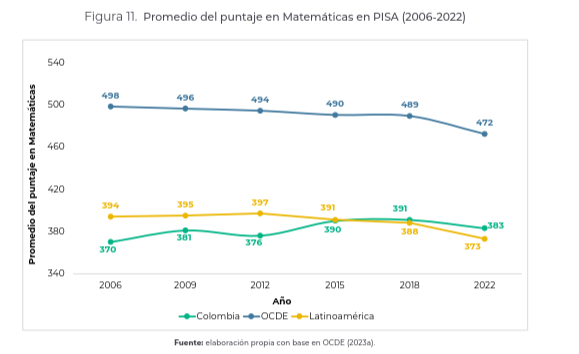
\includegraphics[width=0.88\textwidth]{imagenes/00Figuras/pisa_promedio_puntaje_2006_2022.png}
  \caption{Promedio del puntaje en Matemáticas en PISA (2006--2022) para Colombia, Latinoamérica y la OCDE.
  Tomado de \textcite{icfesProgramaParaEvaluacion2024}.}
  \label{fig:pisa_promedio}
\end{figure}

Más revelador aún es el análisis por niveles de desempeño (Figura~\ref{fig:pisa_niveles}). En 2006, el 72\,\% de los estudiantes colombianos se ubicaba por debajo del nivel~2 —el umbral que la OCDE considera competencia matemática básica—. En 2022, esa cifra era del 71\,\%: dieciséis años de reformas curriculares, nuevos estándares y diversas iniciativas pedagógicas produjeron un desplazamiento de apenas un punto porcentual. En el extremo opuesto, menos del 1\,\% de los estudiantes colombianos alcanza los niveles 5 o~6 —los que corresponden a razonamiento matemático avanzado—, frente al 31\,\% que lo logra en los países de la OCDE. La distribución de desempeño de Colombia en 2022 es prácticamente idéntica a la de 2006.

\begin{figure}[H]
  \centering
  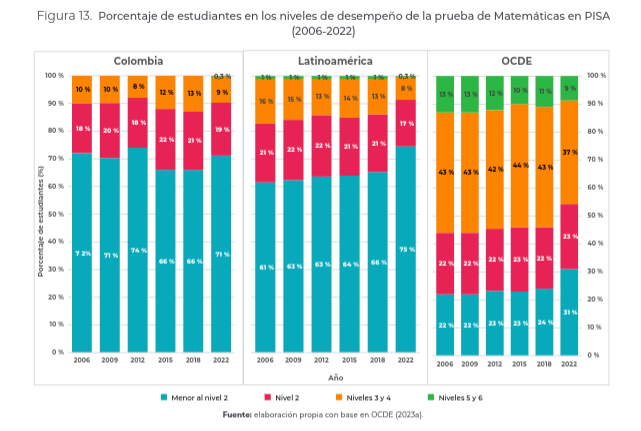
\includegraphics[width=0.88\textwidth]{imagenes/00Figuras/pisa_niveles_desempeno_2006_2022.png}
  \caption{Porcentaje de estudiantes en los niveles de desempeño de la prueba de Matemáticas en PISA (2006--2022). Colombia permanece con más del 70\,\% de estudiantes por debajo del nivel~2 a lo largo de toda la serie.
  Tomado de \textcite{icfesProgramaParaEvaluacion2024}.}
  \label{fig:pisa_niveles}
\end{figure}

Estos datos no implican que el currículo sea erróneo. Implican que el currículo ha prescrito un tipo de razonamiento matemático que las prácticas pedagógicas predominantes no han logrado producir. Una respuesta consistente en la literatura señala la distancia entre lo que el currículo prescribe y lo que efectivamente se desarrolla en el aula.

Los estudios didácticos han documentado que, cuando predominan ejercicios cerrados ---con solución directa y predecible---, se reduce el espacio para la duda, la conjetura y la argumentación. En tales condiciones, el avance en pensamiento matemático profundo es limitado \parencite{fiallolealAcercaInvestigacionEducacion2015,delgadoEstrategiaDidacticaPara2023,zubietaTipificacionErroresDificultades2018}. Modificar esta situación exige rediseñar las tareas para que demanden exploración, comparación de decisiones y análisis del error como parte del aprendizaje.

En este contexto, la IA no se plantea como solución automática, sino como apoyo al diseño didáctico. Puede ofrecer retroalimentación oportuna y abrir rutas diferenciadas según las necesidades del estudiante. Sin embargo, su potencial depende de que la tarea conserve exigencia matemática. Cuando la IA solo automatiza prácticas repetitivas, el aporte pedagógico es mínimo \parencite{romeroalonsoRolInteligenciaArtificial2024,castillodelpezoUseArtificialIntelligence2024,parrasanchezPersonalizacionRecursosPara2023}.

Desde esta perspectiva, el estudio se orienta a comprender qué ocurre cuando se diseñan e implementan tareas de trigonometría con exigencia matemática y apoyo de IA en un contexto escolar real. El interés se centra en identificar qué decisiones didácticas funcionan, dónde aparecen bloqueos y cómo la IA puede aportar sin desplazar el protagonismo del razonamiento matemático del estudiante.


\section{Objetivos}

\subsection{Objetivo general}

Diseñar, implementar y analizar una secuencia de tareas matemáticas que se integran con inteligencia artificial generativa para promover el desarrollo del pensamiento trigonométrico en estudiantes de educación media.

\subsection{Objetivos específicos}

\begin{enumerate}
   
    \item Diseñar una secuencia de tareas matemáticas para educación media, sustentada en criterios didácticos orientados al desarrollo del pensamiento trigonométrico.
   
    \item Integrar una herramienta de inteligencia artificial en el diseño e implementación de la secuencia, de manera que apoye la exploración, la retroalimentación y la argumentación matemática de los estudiantes.

    \item Analizar las evidencias de desarrollo del pensamiento trigonométrico que emergen durante la implementación, considerando estrategias de resolución, dificultades conceptuales y articulación entre representaciones.
\end{enumerate}

\input{capitulos/04_marco_teorico/marco_teorico/marco_teorico.tex}
\section{Marco conceptual}

Este marco no es un catálogo de definiciones. Es una construcción de decisiones: qué tipo de tareas importan para aprendizaje profundo, qué teorías orientan cómo pensamos sobre esas tareas, y cómo la IA puede posicionarse pedagógicamente para expandir —nunca reemplazar— la actividad matemática del estudiante. Las secciones que siguen desarrollan los fundamentos que articulan el diseño de la investigación.

% ─────────────────────────────────────────────────────────────
\subsection{Ejercicio versus tarea: diferencia operativa}
% ─────────────────────────────────────────────────────────────

En las aulas se usa la palabra ``tarea'' para casi cualquier cosa que se pide. Pero esta investigación trabaja con una distinción específica. No es semántica. Es conceptual.

Un \textbf{ejercicio}: el estudiante aplica un procedimiento conocido a situaciones similares. Ejemplo: ``Calcula $\mathrm{sen}(45°)$'' o ``Resuelve $2\mathrm{sen}(x) = 1$ donde $x \in [0, 2\pi]$''. Tiene valor: consolida destreza. Pero encierra el pensamiento. El estudiante reconoce qué fórmula aplicar, hace los pasos, obtiene respuesta. Eso es automatización de procedimientos. No necesariamente comprensión conceptual profunda.

Una \textbf{tarea}: requiere exploración. Ejemplo: ``Un arquitecto diseña una rampa de acceso con ángulo máximo de $30°$. El espacio vertical disponible es 1{,}5 metros. ¿Cuál es la longitud mínima de la rampa? Dibuja la situación, justifica qué razón trigonométrica usaste y explica por qué tu respuesta tiene sentido en contexto.'' Aquí el estudiante no puede simplemente reconocer y aplicar una fórmula. Necesita interpretar contexto, decidir qué representación elegir (dibujo, ecuación, tabla), coordinar conceptos (ángulo, distancia, relación trigonométrica) y justificar la decisión. Exige pensamiento genuino \parencite{leungDesigningMathematicsTasks2015, radmehrTheoreticalFrameworkTask2023, canogullariTaskDesignPrinciples2025}.

Esta distinción orienta el diseño de la investigación: las actividades propuestas no son ejercicios. Son problemas auténticos que requieren razonamiento trigonométrico real.

% ─────────────────────────────────────────────────────────────
\subsection{La trigonometría: recorrido histórico y currículo colombiano}
% ─────────────────────────────────────────────────────────────

\subsubsection{De razón geométrica a función matemática}

La trigonometría no siempre fue lo que es hoy. Su historia es el recorrido de un concepto que nació como herramienta de medición geométrica y se transformó paulatinamente en una familia de funciones matemáticas con dominio en los reales. Comprender ese recorrido ilumina directamente por qué los estudiantes tienen dificultades con la trigonometría escolar: la mayoría de los obstáculos conceptuales que enfrentan hoy son los mismos que la disciplina tuvo que superar históricamente.

En la tradición griega clásica, Hiparco (siglo II a.C.) y Ptolomeo (siglo II d.C.) desarrollaron tablas de cuerdas —no de senos— para calcular posiciones astronómicas. La unidad de medida era la cuerda de un arco en un círculo, no una razón entre lados de un triángulo. La matemática india del siglo V, con Aryabhata, introdujo la \emph{ardha-jya} (semiacuerda), concepto más cercano al seno moderno, que los matemáticos árabes medievales tradujeron y transmitieron a Europa bajo el nombre \emph{sinus} \parencite[p.~311]{katzCalculusTrigonometricFunctions1987}.

El salto conceptual decisivo ocurrió en el siglo XVIII con Euler, quien redefinió las funciones trigonométricas no como razones geométricas sino como funciones de variable real asociadas al círculo unitario. Con Euler, $\mathrm{sen}(x)$ dejó de ser ``el cateto opuesto sobre la hipotenusa en un triángulo rectángulo'' para convertirse en la coordenada $y$ del punto del círculo unitario determinado por el ángulo $x$. Esa redefinición abrió la puerta a tratar las funciones trigonométricas con las herramientas del análisis: derivadas, integrales, series de potencias, extensión a los complejos \parencite{maorTrigonometricDelights1998}.

Esta historia no es anecdótica. El currículo escolar tiende a replicar la trayectoria histórica: primero razones en triángulo rectángulo, luego extensión al círculo unitario, luego funciones periódicas en el plano cartesiano. Cada transición exige del estudiante una reestructuración conceptual —y es en esas transiciones donde emergen los obstáculos más persistentes. Saber que esos obstáculos también marcaron el desarrollo histórico de la disciplina ayuda al docente a anticiparlos en lugar de sorprenderse ante ellos.

La Figura~\ref{fig:circulo_unitario} muestra la relación fundamental que articula las tres fases del desarrollo conceptual: el seno y el coseno como coordenadas del punto $P$ en el círculo unitario para un ángulo $\theta$.

\begin{figure}[H]
\centering
\begin{tikzpicture}[scale=2.8, font=\small]
  % Ejes
  \draw[->] (-1.25,0) -- (1.35,0) node[right] {$x$};
  \draw[->] (0,-1.25) -- (0,1.35) node[above] {$y$};
  % Círculo unitario
  \draw[thick] (0,0) circle (1);
  % Ángulo y radio
  \def\ang{52}
  \draw[thick, blue!70!black] (0,0) -- ({cos(\ang)},{sin(\ang)});
  % Proyecciones
  \draw[dashed, red!70!black, thick] ({cos(\ang)},0) -- ({cos(\ang)},{sin(\ang)});
  \draw[dashed, green!55!black, thick] (0,0) -- ({cos(\ang)},0);
  % Arco del ángulo
  \draw[thick] (0.28,0) arc (0:\ang:0.28);
  \node at ({0.36*cos(\ang/2)},{0.36*sin(\ang/2)}) {$\theta$};
  % Punto P
  \fill[blue!70!black] ({cos(\ang)},{sin(\ang)}) circle (1.2pt);
  \node[right=3pt, blue!70!black] at ({cos(\ang)},{sin(\ang)})
    {$P\!\bigl(\cos\theta,\;\mathrm{sen}\,\theta\bigr)$};
  % Etiquetas proyecciones
  \node[red!70!black, right=3pt] at ({cos(\ang)}, {sin(\ang)/2})
    {$\mathrm{sen}(\theta)$};
  \node[green!55!black, below=3pt] at ({cos(\ang)/2}, 0)
    {$\cos(\theta)$};
  % Marcas de escala
  \foreach \v in {-1,1} {
    \draw (\v, 1.5pt) -- (\v,-1.5pt);
    \draw (1.5pt,\v) -- (-1.5pt,\v);
  }
  \node[below left] at (1,0) {$1$};
  \node[below right] at (-1,0) {$-1$};
  \node[above right] at (0,1) {$1$};
  \node[below right] at (0,-1) {$-1$};
  \node[below left=1pt] at (0,0) {$O$};
\end{tikzpicture}
\caption{Círculo unitario: el seno y el coseno como coordenadas del punto $P$ para el ángulo $\theta$.
La extensión de razón en triángulo rectángulo a coordenada en círculo unitario es el paso conceptual
central que articula el currículo de trigonometría en educación media. Elaboración propia.}
\label{fig:circulo_unitario}
\end{figure}

\subsubsection{La trigonometría en el currículo colombiano}

El currículo colombiano de matemáticas ha evolucionado de forma continua en los últimos treinta años, y esa evolución tiene consecuencias directas para la enseñanza de la trigonometría. No se trata solo de qué contenidos se incluyen, sino de qué tipo de razonamiento se espera que los estudiantes desarrollen y con qué propósito.

Los \emph{Lineamientos Curriculares} \parencite{ministeriodeeducacionnacionalLineamientosCurriculares1998} establecieron el \emph{pensamiento variacional} como uno de los cinco tipos de pensamiento matemático que los estudiantes colombianos deben desarrollar a lo largo de su escolaridad. Dentro de ese pensamiento, las funciones trigonométricas ocupan un lugar central: son el ejemplo canónico de función que describe variación periódica, y su comprensión exige exactamente la articulación entre representación gráfica, algebraica, numérica y contextual que los lineamientos proponen. Esta fue una decisión curricular significativa: posicionó la trigonometría no como técnica de cálculo aislada sino como parte de un programa más amplio de comprensión de la variación matemática.

Los \emph{Estándares Básicos de Competencias} \parencite{ministeriodeeducacionnacionalEstandaresBasicos2006} precisaron ese propósito en estándares observables para los grados décimo y undécimo. Entre ellos: ``Describo y modelo fenómenos periódicos del mundo real usando funciones trigonométricas''. Ese estándar conecta la trigonometría con el mundo real —mareas, movimiento circular, variación térmica— y exige que el estudiante no solo calcule sino que \emph{interprete} y \emph{justifique}. Es el tipo de competencia que no puede evaluarse con un ejercicio rutinario.

Los \emph{Derechos Básicos de Aprendizaje} (DBA) \parencite{ministeriodeeducacionnacionalDerechosBasicos2016} para el grado décimo precisan los aprendizajes concretos esperados: reconocer la amplitud, el período y el desplazamiento de fase de una función trigonométrica; interpretar esos parámetros en contexto; usar el modelo para hacer predicciones verificables. Esos aprendizajes son exactamente los que las dos tareas diseñadas en esta investigación buscan desarrollar y documentar.

Sin embargo, hay una brecha documentada entre lo que el currículo prescribe y lo que ocurre en las aulas. La enseñanza efectiva de la trigonometría en Colombia sigue anclada con frecuencia al procedimiento de razones en triángulos rectángulos, sin alcanzar el nivel funcional y de modelación que los documentos curriculares proponen \parencite{montiel-espinosaDesarrolloPensamientoTrigonometrico2013}. Cerrar esa brecha —diseñando tareas que hagan posible el nivel de pensamiento que el currículo exige— es uno de los propósitos centrales de esta investigación.

% ─────────────────────────────────────────────────────────────
\subsection{Pensamiento trigonométrico}
% ─────────────────────────────────────────────────────────────

Es posible resolver ejercicios de trigonometría sin pensar realmente en trigonometría \parencite{montiel-espinosaDesarrolloPensamientoTrigonometrico2013}. Un estudiante aplica fórmulas, manipula ecuaciones, obtiene respuestas correctas, y aún así no comprende qué representa un seno o coseno más allá de una razón en triángulo rectángulo. El pensamiento trigonométrico genuino va más allá.

Para esta investigación, el pensamiento trigonométrico emerge cuando el estudiante:

\textbf{Primero}, interpreta funciones trigonométricas como objetos funcionales. No como procedimientos (``seno es cateto opuesto sobre hipotenusa''), sino como funciones que describen variación periódica. Significa entender que $y = \mathrm{sen}(x)$ es una relación donde $x$ (el ángulo) es variable independiente e $y$ depende de $x$. Cuando grafica esa relación, ve cómo cambia, interpreta dominio y rango, comprende por qué se repite. Eso es pensamiento funcional sobre trigonometría.

\textbf{Segundo}, articula múltiples representaciones. Una función trigonométrica puede expresarse algebraicamente (ecuación como $y = 2\,\mathrm{sen}(x - \pi/4) + 1$), gráficamente (como curva en el plano), numéricamente (tabla de valores) y verbalmente (``temperatura oscila alrededor de 20°C con amplitud 5° y período 24 horas''). Un estudiante con pensamiento trigonométrico genuino no se queda en un único registro. Puede traducir entre ellos, explicar por qué cada representación resalta aspectos diferentes, usar cada una según el propósito. Esa coordinación requiere esfuerzo y no ocurre espontáneamente \parencite{duval2006}.

\textbf{Tercero}, razona sobre variación y periodicidad con significado. Cuando un problema dice ``función tiene amplitud 3 y período $\pi/2$'', un estudiante sin pensamiento trigonométrico repite palabras sin interpretarlas. Un estudiante con pensamiento trigonométrico explica: amplitud 3 significa oscilación entre $-3$ y $3$; período $\pi/2$ significa que la función completa un ciclo cada $\pi/2$ unidades. Cuando el contexto lo pide, conecta: si el período es $\pi/2$ y representa tiempo en horas, el fenómeno se repite cada $\pi/2$ horas.

\textbf{Cuarto}, diferencia y elige adecuadamente entre radianes y grados. Sabe que ambos son sistemas de medida angular. Entiende que los radianes miden el ángulo en términos del arco en el círculo unitario, mientras los grados dividen el círculo en 360 partes arbitrarias. Cuando trabaja con funciones trigonométricas —donde radianes son el sistema estándar del análisis matemático—, los usa. Cuando el contexto lo requiere, convierte. Esa flexibilidad es signo de pensamiento conceptual.

\textbf{Quinto}, argumenta matemáticamente sobre situaciones problemáticas. No solo resuelve. Además explica por qué su método funciona, qué supuestos hizo, cuáles serían las limitaciones si las condiciones cambiaran, cómo sabe que la respuesta tiene sentido \parencite{montiel-espinosaDesarrolloPensamientoTrigonometrico2013}.

Estas cinco características no son abstractas. Son observables en el aula cuando un estudiante resuelve una tarea: en cómo dibuja la situación, qué expresa algebraicamente, cómo explica sus decisiones, cómo valida la respuesta.

% ─────────────────────────────────────────────────────────────
\subsection{Desarrollo escolar de funciones trigonométricas}
% ─────────────────────────────────────────────────────────────

Las funciones trigonométricas tienen una estructura lógica donde algunas ideas deben preceder a otras \parencite{hsuReviewMathematicalTasks2023}.

Para esta investigación, el desarrollo se estructura en tres fases conectadas, cuya articulación se ilustra en la Figura~\ref{fig:funcion_seno}.

\textbf{Primera fase}: la razón trigonométrica en triángulo rectángulo como fundación. Un estudiante que comprende que en un triángulo rectángulo el seno de un ángulo es la razón entre cateto opuesto e hipotenusa tiene una base. Pero esa base es limitada: funciona solo con ángulos agudos, solo en triángulos rectángulos. El objetivo es que el estudiante sea consciente de esa limitación.

\textbf{Segunda fase}: extensión del concepto al círculo unitario. El triángulo rectángulo entra en un círculo. El ángulo ya no está restringido; puede ser cualquier valor real. La hipotenusa siempre mide 1 (por eso ``unitario''). Ahora el seno de cualquier ángulo es la coordenada $y$ del punto donde el lado terminal del ángulo intersecta el círculo. Eso es crucial: seno deja de ser solo razón y empieza a ser coordenada. La interpretación cambia.

\textbf{Tercera fase}: funciones trigonométricas en el plano cartesiano. Si varío el ángulo de forma continua y trazo los puntos $(x,\, \mathrm{sen}(x))$, obtengo una curva. Esa curva es periódica, oscila, tiene amplitud y período. Se pasa de punto a curva, de valor aislado a función, de estática a variación continua. Los parámetros $A$, $B$, $C$ y $D$ en la expresión $y = A\,\mathrm{sen}(Bx + C) + D$ tienen significado geométrico y contextual preciso.

Estos tres niveles no deben enseñarse desconectados. Un estudiante que ve triángulos rectángulos durante semanas, luego salta al círculo unitario, luego a gráficas, experimentará rupturas conceptuales. Las tareas deben diseñarse para conectar esos niveles, mostrando cómo la razón en triángulo se extiende a coordenada en círculo y luego a función continua en el plano \parencite{montiel-espinosaDesarrolloPensamientoTrigonometrico2013}.

\begin{figure}[H]
\centering
\begin{tikzpicture}
\begin{axis}[
  width=13cm, height=6.5cm,
  axis lines=center,
  xlabel={$x$},
  ylabel={$y$},
  xlabel style={at={(ticklabel* cs:1)}, anchor=west},
  ylabel style={at={(ticklabel* cs:1)}, anchor=south},
  xmin=-0.4, xmax=13.5,
  ymin=-3.8, ymax=4.5,
  xtick={1.5708, 3.1416, 4.7124, 6.2832, 7.8540, 9.4248, 10.9956, 12.5664},
  xticklabels={$\frac{\pi}{2}$, $\pi$, $\frac{3\pi}{2}$, $2\pi$,
               $\frac{5\pi}{2}$, $3\pi$, $\frac{7\pi}{2}$, $4\pi$},
  ytick={-3,-2,-1,1,2,3},
  samples=300,
  smooth,
  tick label style={font=\small},
  label style={font=\small},
  grid=none,
]
  % Línea central D
  \addplot[gray!50, dashed, thick, domain=-0.3:13.3] {0.5};

  % Función y = 2.5·sen(x) + 0.5
  \addplot[blue!70!black, very thick, domain=0:12.8] {2.5*sin(deg(x))+0.5};

  % Anotaciones de amplitud
  \draw[<->, red!70!black, thick]
    (axis cs:1.5708, 0.5) -- (axis cs:1.5708, 3.0)
    node[midway, right=3pt, font=\small] {$A$};

  % Anotación del período
  \draw[<->, green!50!black, thick]
    (axis cs:0.0, -3.5) -- (axis cs:6.2832, -3.5)
    node[midway, below=3pt, font=\small] {$T = \dfrac{2\pi}{B}$};

  % Etiqueta D
  \node[gray!70!black, right=2pt, font=\small] at (axis cs:13.0, 0.5) {$D$};

  % Etiqueta función
  \node[blue!70!black, font=\small] at (axis cs:9.8, 3.4)
    {$y = A\,\mathrm{sen}(Bx + C) + D$};
\end{axis}
\end{tikzpicture}
\caption{Función $y = A\,\mathrm{sen}(Bx + C) + D$ con sus parámetros fundamentales.
La amplitud $A$ determina la magnitud de la oscilación respecto a la línea media $D$;
el período $T = 2\pi/B$ determina la longitud del ciclo completo;
el desfase $C$ desplaza horizontalmente la función.
Comprender el significado contextual de cada parámetro es el objetivo central
de las tareas de esta investigación. Elaboración propia.}
\label{fig:funcion_seno}
\end{figure}

% ─────────────────────────────────────────────────────────────
\subsection{Errores y obstáculos}
% ─────────────────────────────────────────────────────────────

\textcite{brousseauTheoryDidacticalSituations2002} acuñó el término \emph{obstáculo epistemológico} para describir errores que no son meras faltas de atención sino que surgen de una comprensión incompleta que el estudiante debe superar activamente. En trigonometría, estos obstáculos son reales y documentados.

Cuando un estudiante confunde razón con función, ese error no es casualidad. Surge porque está aplicando una interpretación que funciona en el contexto restringido del triángulo rectángulo pero no en el contexto ampliado de las funciones periódicas. El error es una manifestación de que el estudiante todavía no ha integrado los dos marcos conceptuales. Cuando el error se hace visible en una tarea, se discute, y se contrasta con estrategias alternativas que sí funcionan en el contexto general, hay oportunidad de que el estudiante reestructure su comprensión.

Si el error se oculta o se penaliza sin discusión, el estudiante lo repite. La investigación en educación matemática es consistente al respecto \parencite{brousseauTheoryDidacticalSituations2002, arhinAnalysisHighSchool2021}: los errores gestionados productivamente son oportunidades de aprendizaje más valiosas que respuestas correctas acríticas.

Los obstáculos más documentados en trigonometría escolar son:

\begin{itemize}
\item \textbf{Confusión razón–función:} el estudiante aplica $\mathrm{sen}(\theta) = \text{CO}/\text{H}$ en contextos donde la función trigonométrica describe variación continua, no una razón fija en un triángulo específico.
\item \textbf{Interpretación incorrecta de la amplitud:} confundir el valor máximo de la función con la amplitud, o no reconocer la amplitud como la distancia entre el valor máximo y la línea media.
\item \textbf{Errores en el período:} confundir el coeficiente $B$ directamente con el período, sin aplicar la relación $T = 2\pi/B$.
\item \textbf{Dificultades con los radianes:} operar mecánicamente entre grados y radianes sin comprender que son dos formas de medir el mismo ángulo.
\item \textbf{Desconexión parámetro–contexto:} calcular correctamente los parámetros de una función sin poder interpretar qué significan en la situación física que modelan.
\end{itemize}

Las tareas de esta investigación están diseñadas para hacer visibles estos obstáculos. No para evitarlos, sino para provocar que emerjan y puedan ser examinados \parencite{leungDesigningMathematicsTasks2015}.

% ─────────────────────────────────────────────────────────────
\subsection{GeoGebra y génesis instrumental}
% ─────────────────────────────────────────────────────────────

Durante décadas, la matemática se enseñó con papel y pizarrón. El estudiante llenaba cuadernos con gráficas trazadas a mano, cálculos mecánicos, ecuaciones copiadas. Las herramientas como GeoGebra transforman esa experiencia de forma fundamental: no son simplemente un crayón digital. Cuando un estudiante mueve un deslizador que controla la amplitud de una función seno, la gráfica responde en tiempo real. Ve que amplitud 2 produce una oscilación entre $-2$ y $2$, que amplitud 5 la extiende entre $-5$ y $5$. No memorizado. Visto. Experimentado. \parencite{hohenwartherCombinationDynamicGeometry2004, zenginEffectDynamicMathematics2012}.

Sin embargo, la mera disponibilidad de una herramienta potente no garantiza aprendizaje. \textcite{troucheManagingComplexityHuman2004} desarrolló el concepto de \emph{génesis instrumental} para distinguir entre un \emph{artefacto} (el software tal como existe, independientemente del usuario) y un \emph{instrumento} (el artefacto integrado en la actividad del sujeto a través del uso). GeoGebra no es automáticamente un instrumento para quien lo usa por primera vez. Se convierte en instrumento en la medida en que el estudiante desarrolla esquemas de uso: sabe qué herramientas usar para qué propósito, cómo interpretar los resultados, cuándo confiar en la representación gráfica y cuándo el cálculo algebraico es más preciso.

Esta distinción tiene implicaciones directas para el diseño de las tareas. Una tarea que pide ``grafica la función que el docente dicta en GeoGebra'' mantiene a los estudiantes en el nivel del artefacto: usan el software mecánicamente, sin desarrollar comprensión sobre lo que están representando. Una tarea que pide ``explora qué sucede con la gráfica cuando cambias el parámetro $B$; describe el patrón que observas y formula una conjetura'' usa GeoGebra como instrumento pedagógico: el software amplía el espacio de observación y el estudiante debe pensar sobre lo que ve.

La Figura~\ref{fig:circulo_unitario} (ya incluida en la sección anterior) ilustra la representación que GeoGebra permite explorar de forma dinámica: el punto $P$ sobre el círculo unitario que se mueve al variar el ángulo $\theta$, y las proyecciones que definen el seno y el coseno como coordenadas. En papel, esa relación se ve como un diagrama estático. En GeoGebra, el estudiante puede mover el punto y observar cómo las proyecciones cambian continuamente.

% ─────────────────────────────────────────────────────────────
\subsection{IA generativa como agente de acompañamiento matemático}
% ─────────────────────────────────────────────────────────────

La inteligencia artificial generativa —en particular los modelos de lenguaje de gran escala como ChatGPT— ha comenzado a ingresar al espacio educativo de formas heterogéneas: como fuente de explicaciones, como generador de ejercicios, como tutor conversacional, o simplemente como herramienta para eludir el trabajo matemático. El uso pedagógico genuino exige posicionarla con claridad \parencite{castillodelpezoUseArtificialIntelligence2024}.

Para esta investigación, ChatGPT no es una calculadora avanzada ni un repositorio de respuestas. Es un \emph{agente de acompañamiento matemático}: un interlocutor con quien el estudiante puede dialogar sobre sus ideas, contrastar sus conjeturas, recibir preguntas que lo obliguen a precisar su razonamiento, y explorar caminos alternativos de solución. Ese posicionamiento pedagógico no es accidental: se implementa mediante instrucciones explícitas en el sistema de la herramienta que definen qué puede y qué no puede hacer la IA en el contexto de las tareas.

Investigaciones recientes sobre ChatGPT en educación matemática documentan un patrón consistente \parencite{wardatChatGPTRevolutionaryTool2023}: cuando los estudiantes usan la herramienta para que les dé la respuesta, el aprendizaje no ocurre. Cuando la usan para explorar, para verificar hipótesis, para recibir retroalimentación sobre su propio trabajo, el potencial pedagógico aumenta significativamente. La distinción no está en la herramienta sino en cómo está posicionada dentro de la tarea.

Como señala \textcite{pepinMathematicsEducationEra2025}: la IA entra en la actividad matemática del estudiante, devuelve información y orienta decisiones. Su valor educativo no viene del software sino de cómo se integra en el diseño de la tarea. Una IA en una tarea de alta exigencia matemática —donde el estudiante ya debe razonar, explorar y justificar— expande las oportunidades de pensamiento. La misma IA en una tarea mecánica convierte el aprendizaje en una búsqueda de respuestas.

Por eso, en esta investigación, la IA no ocupa el centro. El pensamiento matemático sí. La IA funciona como apoyo deliberado para ese pensamiento cuando la tarea está diseñada adecuadamente.

% ─────────────────────────────────────────────────────────────
\subsection{Síntesis}
% ─────────────────────────────────────────────────────────────

Diseñar tareas con IA generativa que resulten didácticamente efectivas para el desarrollo del pensamiento trigonométrico exige sostener cinco dimensiones simultáneamente:

\textbf{Primero}, fundamentación histórica y curricular: las tareas deben articularse con el recorrido conceptual que la disciplina y el currículo colombiano proponen, no ignorarlo.

\textbf{Segundo}, exigencia matemática real: lo solicitado debe requerir razonamiento genuino, no reproducción de procedimientos. El estudiante debe explorar, decidir, justificar.

\textbf{Tercero}, articulación de representaciones: las tareas deben crear condiciones para que el estudiante transite entre registros —gráfico, algebraico, numérico, contextual— no que se quede atrapado en uno solo.

\textbf{Cuarto}, uso instrumental de GeoGebra: la herramienta debe integrarse como instrumento que amplía el espacio de observación, no como crayón digital que grafica lo que el docente dicta.

\textbf{Quinto}, posicionamiento pedagógico explícito de la IA: ChatGPT funciona como agente de acompañamiento que provoca pensamiento, no como solucionador que lo reemplaza.

Si una de estas dimensiones falla, la IA tiende a ocupar un protagonismo que desplaza el objetivo formativo y debilita el desarrollo del pensamiento trigonométrico.

\section{Marco referencial}
\label{sec:marco_referencial}

Dos tipos de referentes delimitan esta investigación: el marco curricular colombiano vigente para la educación media, y los referentes internacionales en diseño de tareas matemáticas que orientan sus decisiones pedagógicas.

\subsection{Marco curricular colombiano}

Como objeto matemático, la trigonometría no se agota en el triángulo rectángulo. También articula medición angular, periodicidad y modelación de fenómenos cíclicos, por lo que conecta la geometría con el análisis matemático y con múltiples aplicaciones científicas y tecnológicas.

Los \emph{Lineamientos Curriculares de Matemáticas} ubican la trigonometría en relación con el pensamiento variacional, la modelación y el análisis de fenómenos de cambio \parencite{ministeriodeeducacionnacionalLineamientosCurriculares1998}. Los \emph{Estándares Básicos de Competencias} van más allá: en décimo y undécimo, los estudiantes deben interpretar el comportamiento de funciones, relacionar parámetros algebraicos con representaciones gráficas y modelar situaciones periódicas del mundo real \parencite{ministeriodeeducacionnacionalEstandaresBasicos2006}. Y los \emph{Derechos Básicos de Aprendizaje} cierran el círculo insistiendo en la comprensión funcional y en el uso flexible de representaciones, no solo en la ejecución de procedimientos algorítmicos \parencite{ministeriodeeducacionnacionalDerechosBasicos2016}.

Ese marco normativo sustenta la decisión de centrar el estudio en el pensamiento trigonométrico y en el diseño de tareas con integración de IA generativa. No es solo normativo, sin embargo. También incorpora estudios que documentan dificultades recurrentes en trigonometría escolar —el tránsito de razón trigonométrica a función, la interpretación de la periodicidad, la articulación de registros semióticos \parencite{delgadoEstrategiaDidacticaPara2023, chaconComprensionRazonesTrigonometricas2007, zubietaTipificacionErroresDificultades2018}—, y esos hallazgos operan como criterio para seleccionar y diseñar las tareas de la investigación.

\subsection{Referentes internacionales en diseño de tareas matemáticas}

¿Qué hace que una tarea matemática genere aprendizaje real, en vez de solo ocupar el tiempo de la clase? Esa pregunta atraviesa la literatura internacional sobre diseño de tareas, y tres referentes la responden desde ángulos distintos —cada uno completando lo que el anterior deja sin resolver.

\textbf{NCTM (2014)} ofrece una primera respuesta, centrada en la demanda cognitiva. \emph{Principles to Actions} \parencite{nctmPrinciplesActions2014} distingue cuatro niveles —memorización, procedimientos sin conexión, procedimientos con conexión, y hacer matemáticas— y sostiene que la instrucción de calidad exige sostenerse en los dos niveles superiores. Es un criterio útil. Pero deja una pregunta sin responder: ¿de dónde sale ese espacio de exploración que una tarea de alta demanda necesita para funcionar? Este referente sustenta, de todos modos, la distinción ejercicio/tarea que articula el marco conceptual de la investigación.

Ahí entra \textbf{Watson y Ohtani (2015)}. El estudio de la ICMI sobre diseño de tareas \parencite{watsonTaskDesignMathematics2015} sintetiza décadas de investigación y precisa algo que el criterio de NCTM da por sentado: ese espacio de posibilidades matemáticas no está en el enunciado de la tarea. Está en las herramientas disponibles, el tiempo, las interacciones con pares y con el docente, los recursos tecnológicos. Para esta investigación, esa precisión es directamente operativa: ChatGPT y GeoGebra no son accesorios del enunciado. Son parte de ese espacio.

Falta todavía una pieza: ¿qué es exactamente lo que ese espacio de exploración intenta mover en la cabeza del estudiante? \textbf{Sfard (1991)} \parencite{sfardDualNatureMathematical1991} responde con la distinción entre concepción operacional —el objeto matemático como proceso o algoritmo— y estructural —como objeto estático, con propiedades. El tránsito entre ambas es uno de los desafíos cognitivos más importantes del aprendizaje matemático avanzado, y la trigonometría lo ilustra con particular claridad: el seno puede ser un procedimiento para calcular razones en un triángulo, o puede ser una función —periódica, continua, diferenciable— con dominio en los reales. Las tareas de esta investigación se diseñan para mover al estudiante de lo primero hacia lo segundo.

Los tres referentes no compiten entre sí: se completan. NCTM fija el nivel de exigencia. Watson y Ohtani ubican dónde vive ese espacio de exigencia. Sfard nombra la transformación cognitiva que se busca dentro de él.

\section{Marco contextual}
\label{sec:marco_contextual}

La investigación se desarrolla en un contexto de educación media colombiana, con estudiantes de grado décimo y undécimo en una institución educativa de carácter oficial. El interés del estudio se centra en escenarios de aula reales, con condiciones habituales de tiempo, infraestructura y heterogeneidad académica.

En este contexto, la enseñanza de la trigonometría suele concentrarse en unidades curriculares de corta duración y con presión por cobertura de contenidos, lo que frecuentemente reduce el espacio para argumentación y análisis de errores. Esta condición contextual refuerza la necesidad de diseñar tareas que, aun en tiempos limitados, sostengan exigencia matemática y discusión matemática.

También se reconoce una incorporación creciente de recursos digitales en la escuela, aunque con diferencias en acceso, conectividad y familiaridad tecnológica entre estudiantes. Por ello, la integración de IA en esta investigación se plantea de forma gradual, con actividades guiadas y criterios didácticos explícitos, evitando depender de condiciones tecnológicas excepcionales.

El contexto institucional, curricular y tecnológico descrito no se considera un telón de fondo secundario, sino una variable que incide directamente en la viabilidad del diseño de tareas y en la interpretación de los resultados del estudio.


\chapter{Marco metodológico}
\label{chap:marco_metodologico}

\section{Posicionamiento metodológico: el experimento de enseñanza}

Esta investigación adopta el experimento de enseñanza como diseño metodológico. La elección responde a la pregunta que la orienta: ¿cómo diseñar e implementar tareas de trigonometría con inteligencia artificial de manera que contribuyan al desarrollo del pensamiento trigonométrico en estudiantes de grado décimo?

Esa pregunta no se responde midiendo resultados de aprendizaje en dos grupos paralelos. Se responde observando con detenimiento cómo piensan los estudiantes cuando resuelven esas tareas; qué errores cometen y qué revelan sobre su comprensión; cómo interactúan con la IA y qué papel juega esa interacción en su razonamiento; y de qué manera el diseño de las tareas facilita —o no— el tránsito entre representaciones gráficas, algebraicas y contextuales de las funciones trigonométricas.

El experimento de enseñanza ofrece algo que los diseños comparativos no pueden: acceso al pensamiento matemático \emph{mientras se construye} \parencite{steffe2000teaching}. El investigador no observa desde afuera el resultado de un proceso educativo ya terminado. Participa activamente en él: diseña tareas, las implementa con los estudiantes, registra lo que ocurre, y vuelve al diseño con ese conocimiento acumulado. Esa iteratividad no es una característica secundaria del método. Es su lógica central.

\textcite{gonzalezAcercamientoInvestigacionDiseno2011} precisan que en los experimentos de enseñanza el objeto de estudio no es el estudiante en abstracto sino los procesos de aprendizaje matemático en un contexto específico de interacción: con el docente, con las tareas, con las herramientas disponibles. En esta investigación, esa herramienta es la inteligencia artificial generativa. Documentar cómo media el pensamiento trigonométrico —cuándo abre el pensamiento, cuándo lo reemplaza, en qué condiciones resulta andamiaje genuino— es el núcleo del trabajo.

\textcite{cobb2003design} sitúan los experimentos de enseñanza dentro de una familia más amplia de diseños que comparten un rasgo: el objeto de estudio no es independiente del proceso de investigación, sino que se construye a través de él. Las tareas no se diseñan antes de la investigación y se aplican mecánicamente. Se diseñan, se implementan, se analizan, y se rediseñan. Eso es lo que aquí ocurrirá.

\subsection{Por qué no un diseño comparativo}

Una aproximación razonable sería comparar dos grupos: uno con acceso a IA, otro sin acceso. Esa elección tiene valor propio y responde preguntas del tipo: ¿qué diferencias en desempeño o en estrategias emergen cuando se tiene o no se tiene IA disponible?

Pero eso no es lo que aquí interesa. Lo que interesa es comprender \emph{cómo} —bajo qué condiciones de diseño, con qué tipo de consignas, en qué momentos específicos de la secuencia— la IA puede funcionar como agente de acompañamiento matemático que provoca pensamiento en lugar de reemplazarlo. Esa pregunta exige diseño iterativo, observación sostenida, y análisis que capture la particularidad de los procesos. No exige comparación estadística.

\section{Paradigma de investigación}

Esta investigación se posiciona en el paradigma pospositivista \parencite{phillipsBurbules2000, creswell2014research}. El pospositivismo reconoce que existe una realidad —en este caso, el pensamiento trigonométrico de los estudiantes y los procesos de aprendizaje que ocurren en el aula— pero acepta que esa realidad solo puede conocerse de forma aproximada e imperfecta. A diferencia del positivismo clásico, que asume objetividad plena y medición exacta, el pospositivismo reconoce que el investigador influye sobre lo que estudia y que el conocimiento siempre es provisional. A diferencia del paradigma interpretativo, no renuncia a la búsqueda de patrones sistemáticos ni al rigor metodológico como criterio de validez.

Para esta investigación, ese posicionamiento tiene implicaciones concretas. El pensamiento trigonométrico de los estudiantes existe como objeto real —no es construido arbitrariamente por el investigador—, pero solo puede aproximarse a través de múltiples fuentes de datos (observaciones, entrevistas, producciones escritas, registros de interacción con la IA) analizadas con rigor y trianguladas. Ninguna fuente individual ofrece acceso completo a lo que realmente ocurre en la mente del estudiante cuando resuelve una tarea. Las fuentes combinadas permiten aproximaciones más confiables.

\textcite{creswell2014research} señala que el pospositivista trabaja con métodos cualitativos cuando la naturaleza del fenómeno así lo exige: cuando lo que importa comprender es el proceso y no solo el resultado, cuando los participantes son pocos y el contexto es específico, cuando el análisis estadístico no puede capturar lo que se busca. Todas esas condiciones se cumplen aquí.

\textcite{camargoConferenciaInteramericanaEducacion10} precisa que en educación matemática las estrategias de diseño —como el experimento de enseñanza— no buscan neutralidad del investigador sino rigor en la documentación de sus decisiones y sus efectos. El investigador-docente no se borra del proceso. Lo registra sistemáticamente y lo convierte en parte del análisis.

\section{Fundamentación teórica de las decisiones metodológicas}

Tres marcos teóricos orientan las decisiones de diseño, implementación y análisis de este experimento de enseñanza.

\textbf{Pensamiento trigonométrico.} \textcite{montiel-espinosaDesarrolloPensamientoTrigonometrico2013} desarrolla el concepto de pensamiento trigonométrico como la capacidad de transitar entre la representación geométrica del ángulo, la representación funcional de las razones trigonométricas, y la modelación de fenómenos periódicos reales, sin que ninguno de estos registros sea suficiente por sí solo. Ese tránsito es lo que las tareas de esta investigación buscan provocar y lo que el análisis documentará. La pregunta no es si el estudiante sabe la fórmula de la función seno. Es si puede moverse con soltura entre la situación física, la gráfica y la expresión algebraica, y si puede justificar por qué cada parámetro tiene el valor que tiene.

\textbf{Registros de representación semiótica.} \textcite{duval2006} muestra que la comprensión matemática no reside en dominar un registro aislado —la ecuación algebraica, la gráfica, la tabla numérica— sino en coordinar activamente entre ellos. Los errores más persistentes en trigonometría escolar emergen precisamente cuando los estudiantes no logran articular lo que la gráfica dice con lo que la ecuación representa. Las tareas de esta investigación están diseñadas para hacer visible esa articulación —o su ausencia—, y las observaciones registrarán específicamente cuándo y cómo los estudiantes alternan o fallan en alternar entre registros.

\textbf{Diseño de tareas matemáticas.} \textcite{leungDesigningMathematicsTasks2015} identifican criterios para tareas que exigen pensamiento matemático profundo: deben admitir múltiples caminos de solución, conectar con fenómenos reales, y crear las condiciones para que errores conceptuales emerjan y sean examinados. \textcite{radmehrTheoreticalFrameworkTask2023} y \textcite{canogullariTaskDesignPrinciples2025} añaden que una tarea de alta exigencia cognitiva no puede resolverse aplicando directamente una fórmula memorizada: exige explorar, comparar estrategias y justificar decisiones. Ese criterio rige el diseño de las dos tareas de esta investigación.

La inteligencia artificial entra en este marco no como tema de estudio sino como herramienta de mediación. Su rol no es entregar respuestas correctas. Es funcionar como agente de acompañamiento que el estudiante interroga, evalúa y contrasta con sus propias construcciones. Este criterio —que la IA nunca resuelva directamente sino que provoque pensamiento— es la apuesta pedagógica central del diseño, y documentar cuándo se cumple y cuándo no es uno de los objetivos del análisis.

\section{Diseño del experimento de enseñanza}

\subsection{El docente-investigador}

En el experimento de enseñanza, el investigador no es un observador externo. Es, al mismo tiempo, quien diseña las tareas, las implementa con los estudiantes, registra lo que ocurre, y utiliza ese conocimiento para refinar el diseño. \textcite{steffe2000teaching} denominan a esta figura el \emph{teacher-researcher}: alguien que actúa pedagógicamente y analiza simultáneamente.

Eso tiene implicaciones concretas aquí. Las dos tareas que se describen en este capítulo son la versión actual del diseño. No son definitivas. Si durante la implementación emerge un obstáculo conceptual no anticipado, o si la IA genera un tipo de interacción que modifica el rumbo de la sesión, el diseño se ajustará. Eso no es falta de rigor. Es exactamente lo que el método exige.

\subsection{Contexto e institución}

El experimento se implementa en el Colegio Villa de las Palmas, institución de educación media privada ubicada en Palmira, Valle del Cauca. El municipio cuenta con aproximadamente 300.000 habitantes y se encuentra a 30 km al norte de Cali, en una zona urbana con infraestructura educativa desarrollada.

La institución cuenta con aulas equipadas con computadores e internet, lo que hace técnicamente posible el uso simultáneo de GeoGebra y ChatGPT durante las sesiones de trabajo. Al año 2026, el Colegio Villa de las Palmas tiene una matrícula de 230 estudiantes. La selección de este contexto responde a un criterio práctico y epistemológico a la vez: es la institución donde el investigador ejerce como docente, lo que garantiza acceso sostenido al grupo durante el período de implementación y una familiaridad con el contexto que ningún observador externo podría reemplazar.

\subsection{Participantes}

\textbf{Grupo de trabajo.} Se trabaja con el grupo completo de grado décimo, conformado por 25 estudiantes, cuyas edades oscilan entre 15 y 17 años. Todos los estudiantes del grupo participan en las sesiones de trabajo con las tareas.

\textbf{Muestra intensiva.} Para el análisis más detallado —entrevistas semiestructuradas, análisis de producciones, seguimiento de trayectorias individuales— se seleccionan 4 a 6 estudiantes que representen la diversidad de desempeños del grupo:

\begin{itemize}
  \item Al menos 1-2 estudiantes con desempeño alto en matemáticas.
  \item Al menos 1-2 estudiantes con desempeño medio o variable.
  \item Al menos 1-2 estudiantes con dificultades persistentes en matemáticas.
  \item Representación de ambos géneros en la medida de lo posible.
\end{itemize}

Esta muestra intensiva no es una muestra estadística. Es un mecanismo para documentar en profundidad trayectorias de aprendizaje particulares que ilustren patrones más amplios del grupo.

\subsection{La secuencia de tareas}

Las tareas son el corazón del experimento. Se diseñan dos tareas para la versión inicial de implementación:

\begin{itemize}
  \item \textbf{Tarea 1}: Las transformaciones de la función seno: la rueda de la fortuna.
  \item \textbf{Tarea 2}: Modelar con coseno: el movimiento de las mareas.
\end{itemize}

Ambas tareas responden a cinco criterios didácticos que rigen el diseño \parencite{leungDesigningMathematicsTasks2015, radmehrTheoreticalFrameworkTask2023, canogullariTaskDesignPrinciples2025}:

\begin{enumerate}
  \item \textbf{Exigencia matemática alta}: la tarea no puede resolverse aplicando directamente una fórmula. Exige explorar, comparar estrategias y justificar decisiones.
  \item \textbf{Articulación de representaciones}: cada actividad exige trabajar con al menos dos tipos de representación —gráfica, algebraica, numérica o verbal— y transitar entre ellas \parencite{duval2006}.
  \item \textbf{Rol explícito de la IA}: se define con precisión cuándo y cómo usa el estudiante ChatGPT: para interrogar, contrastar o solicitar retroalimentación; nunca para obtener la respuesta directa de la tarea.
  \item \textbf{Espacio para el error}: las consignas admiten respuestas parciales o erróneas como punto de partida legítimo para la discusión, no como faltas a corregir.
  \item \textbf{Contextualización}: las situaciones conectan con fenómenos periódicos reales —el movimiento de una rueda de la fortuna, las mareas costeras— y tienen sentido fuera del aula de matemáticas.
\end{enumerate}

Cada tarea está organizada en cinco momentos didácticos articulados, cuya secuencia responde a una lógica de construcción progresiva en la que cada momento prepara el siguiente. La Tarea 1 activa el tránsito de la razón trigonométrica a la función seno como objeto matemático propio; la Tarea 2 exige movilizar ese conocimiento para modelar un fenómeno diferente con coseno. El diseño completo de cada tarea, con sus momentos didácticos, errores esperados y criterios de evaluación, se presenta en la sección de métodos y materiales.

\subsection{Ciclos del experimento}

El experimento se organiza en tres ciclos iterativos \parencite{cobb2003design}:

\begin{description}
  \item[Ciclo 1 — Diseño:] Elaboración de las tareas con base en criterios teóricos, revisión de la literatura sobre obstáculos conceptuales en trigonometría, y diseño de instrumentos de recolección de datos (guías de observación, protocolo de entrevistas, rúbrica analítica).
  \item[Ciclo 2 — Implementación y registro:] Aplicación de las tareas con el grupo durante 8 a 10 semanas. Observación sistemática, recolección de producciones escritas, grabaciones de audio o video con consentimiento, y entrevistas con la muestra intensiva.
  \item[Ciclo 3 — Análisis y rediseño:] Análisis del material recolectado, identificación de patrones de razonamiento y obstáculos persistentes, y, si el tiempo y las condiciones lo permiten, rediseño de las tareas con base en los hallazgos para un ciclo posterior.
\end{description}

\section{Recolección de datos}

La recolección se organiza alrededor de documentar cómo los estudiantes abordan las tareas: qué estrategias despliegan, en qué puntos se quedan atrapados, cómo interactúan con la IA, y cómo evoluciona su pensamiento a lo largo de la secuencia.

\textbf{Observación de sesiones.} Durante cada sesión se registra mediante notas de campo lo que ocurre: estrategias que cada estudiante intenta, momentos específicos de bloqueo, preguntas que formula (al docente-investigador o a la IA), representaciones que usa espontáneamente, y manifestaciones de comprensión o confusión. Se documentan especialmente los momentos de consulta a la IA: qué pregunta exacta formula el estudiante, cómo interpreta la respuesta, si cambia de estrategia después. Las sesiones se graban en audio o video cuando sea posible y con consentimiento informado.

\textbf{Entrevistas semiestructuradas.} Con la muestra intensiva (4-6 estudiantes), se realizan entrevistas de 15 a 20 minutos después de que completan conjuntos de tareas. Las conversaciones buscan acceder directamente al pensamiento del estudiante: ¿cuál fue tu primer paso? ¿dónde te atascaste? ¿qué hiciste entonces? ¿cuándo decidiste consultar la IA y por qué? ¿la respuesta que recibiste te resultó útil o te confundió? No se trata de cuestionarios rígidos. El investigador escucha, hace preguntas de seguimiento basadas en lo que el estudiante dice, y evita sugerir respuestas.

\textbf{Producciones de los estudiantes.} Se recolecta y preserva todo lo que escriben y dibujan durante las sesiones: cálculos, gráficos dibujados a mano, tablas de datos, diagramas, borradores con correcciones. Especialmente los borradores: muestran el proceso de pensamiento que la respuesta final borra. También se registran las capturas de las interacciones con ChatGPT. Este material es central para el análisis.

\textbf{Cuestionarios de contexto.} Al inicio se aplica un cuestionario breve (15 minutos) que mide conocimiento previo de trigonometría, autopercepción matemática, y experiencia previa con herramientas de IA. Al final, otro cuestionario de similar extensión mide autopercepción posterior y reflexión sobre la experiencia con la herramienta. Estos cuestionarios no buscan cuantificar aprendizaje. Buscan contexto para interpretar lo que se observó.

\section{Procedimiento de análisis}

El análisis no busca producir números ni verificar hipótesis previas. Busca describir con detalle y rigor cómo piensan realmente estos estudiantes.

\textbf{Fase 1 — Preparación e inmersión.} Se transcribe cada grabación palabra por palabra, se digitalizan fotografías de producciones, y se revisan y amplían las notas de campo. Este acto de organizar ya es análisis: al transcribir emergen patrones; al ampliar notas, se recuperan contextos que los datos brutos no capturan.

\textbf{Fase 2 — Codificación abierta.} Se lee el material sin categorías preconcebidas. La pregunta guía es: ¿qué está ocurriendo realmente aquí? Se marcan episodios relevantes: momentos donde el estudiante muestra comprensión nueva; errores específicos y cómo los intenta corregir; cambios de estrategia; consultas a la IA —qué pregunta exacta, cómo interpreta la respuesta, qué hace después. Las categorías no se fuerzan. Emergen del material.

\textbf{Fase 3 — Codificación axial.} Se agrupan códigos abiertos en categorías mayores. Códigos sobre ``dibuja la situación'', ``construye tabla de valores'' se agrupan bajo ``modos de representación visual''. Se buscan relaciones: ¿existe conexión entre el tipo de error y la estrategia inicial? ¿La IA modificó esa relación?

\textbf{Fase 4 — Análisis de patrones.} Se examinan los patrones emergentes a lo largo de la secuencia completa: ¿cómo evoluciona el pensamiento del Momento 1 al Momento 5? ¿Los obstáculos conceptuales documentados en la literatura —confusión entre amplitud y período, dificultad con el desfase— aparecen con la misma forma que se describe, o se manifiestan de manera diferente en este grupo específico? ¿Cuándo usa el estudiante la IA de forma que expande su razonamiento y cuándo la usa para eludir el pensamiento?

\textbf{Fase 5 — Triangulación.} Se aplican dos tipos de triangulación para fortalecer la credibilidad de los hallazgos \parencite{creswell2014research}:

\textbf{(a) Triangulación de fuentes:} los patrones identificados en las notas de observación se contrastan con las producciones escritas de los estudiantes y con los registros de las entrevistas. Un hallazgo que aparece en las tres fuentes gana credibilidad; una discrepancia entre fuentes —el estudiante afirma que entendió, pero sus cálculos muestran confusión— se examina como dato en sí mismo. Ahí suele estar la comprensión más real.

\textbf{(b) Triangulación de investigador:} los hallazgos preliminares se revisan con los directores de tesis en sesiones de análisis conjunto, reduciendo el riesgo de sesgos interpretativos del investigador-docente. Esta revisión es especialmente necesaria dado que el investigador es también quien implementó las tareas y conoce personalmente a los estudiantes.

\textbf{Fase 6 — Narrativas analíticas.} El producto final no es un listado de códigos ni una tabla de frecuencias. Son narrativas que explican cómo piensan realmente los estudiantes. Con estructura. Con ejemplos específicos tomados del material. Con reconocimiento explícito de lo que no puede concluirse. Ese es el tipo de conocimiento que esta investigación busca producir.

\section{Ubicación del proyecto}
\label{sec:ubicacion_proyecto}

\subsection{Localización geográfica e institucional}

La investigación se desarrolla en el Colegio Villa de las Palmas, institución educativa privada de educación media ubicada en Palmira, Valle del Cauca, Colombia. Palmira es un municipio ubicado en el norte del departamento del Valle del Cauca, aproximadamente a 30 kilómetros de Cali, con una población de cerca de 300,000 habitantes.

El Colegio Villa de las Palmas atiende estudiantes de educación básica secundaria y educación media. Al año 2026 cuenta con una matrícula de 230 estudiantes, distribuidos en los niveles de sexto a undécimo grado. La institución dispone de aulas equipadas con computadores e internet, acceso a recursos tecnológicos, y apertura de la administración para facilitar el desarrollo de investigaciones educativas en sus instalaciones.

\subsection{Población estudiantil}

La población de referencia son estudiantes de grados décimo y undécimo del colegio. Esta población fue seleccionada por varias razones:

\begin{enumerate}
\item \textbf{Madurez cognitiva:} Estudiantes en edades entre 15 y 17 años se encuentran en etapa de pensamiento formal, con capacidades de abstracción y razonamiento lógico-matemático desarrolladas.

\item \textbf{Familiaridad con trigonometría:} Es en décimo y undécimo donde se enseña trigonometría formalmente en el currículo colombiano, por lo que estos estudiantes tienen acceso a instrucción sistemática en el tema.

\item \textbf{Experiencia con tecnología:} Estudiantes de esta edad típicamente tienen experiencia previa con herramientas digitales, lo que reduce la curva de aprendizaje asociada al uso de la herramienta de IA.

\item \textbf{Disponibilidad temporal:} Es posible coordinar con la institución sesiones de trabajo regulares dentro de horario académico.
\end{enumerate}

\subsection{Cronología de la implementación}

La implementación está planeada para una duración de 8 a 10 semanas, distribuidas a lo largo de un período académico semestral. Esto permite:

\begin{itemize}
\item Sesiones de trabajo regulares con estudiantes (idealmente 2-3 sesiones por semana de 45-60 minutos cada una).
\item Tiempo suficiente para que los estudiantes completen un conjunto coherente de tareas trigonométricas.
\item Espacio para entrevistas con estudiantes seleccionados sin interrumpir demasiado el horario de clases.
\item Período de análisis de datos al final sin presión de tiempo extrema.
\end{itemize}

La cronología específica se coordina con la institución considerando calendarios académicos, períodos de evaluación, y disponibilidad de espacios físicos.

\subsection{Justificación de la selección del sitio}

Se seleccionó el Colegio Villa de las Palmas por:

\begin{enumerate}
\item \textbf{Accesibilidad:} La institución está dispuesta a permitir la investigación y facilitar acceso a estudiantes y espacios.

\item \textbf{Características pedagógicas:} Existe disposición del docente de matemáticas a participar, coordinando la implementación sin que esto interfiera significativamente con el currículo regular.

\item \textbf{Composición estudiantil:} La población es heterogénea en términos de desempeño académico en matemáticas, lo que permite documentar cómo estudiantes con distintos niveles de competencia se relacionan con la IA.

\item \textbf{Recursos tecnológicos:} El colegio tiene acceso a computadores y conectividad, lo que permite que el grupo experimental tenga acceso confiable a la herramienta de IA.

\item \textbf{Contexto socioeconómico:} Los estudiantes provienen de contextos socioeconómicos medios, lo que implica familiaridad previa con tecnología pero no ``natividad digital'' extrema que pudiera sesgar los resultados.
\end{enumerate}

\section{Métodos y materiales}
\label{sec:metodos_materiales}

\subsection{Participantes y criterios de selección}

\subsubsection{Grupo de trabajo}

El estudio involucra el grupo completo de grado décimo del Colegio Villa de las Palmas: 25 estudiantes, con edades entre 15 y 17 años. La institución cuenta con 230 estudiantes en total al año 2026.

Los criterios de inclusión son:

\begin{itemize}
\item Estar matriculado en grado décimo en el colegio durante el período de implementación.
\item Contar con presencia durante las sesiones de trabajo (8-10 semanas).
\item Consentimiento informado del estudiante y del acudiente.
\end{itemize}

\subsubsection{Muestra intensiva}

Dentro del grupo, se seleccionan 4 a 6 estudiantes para un seguimiento más profundo. Esta muestra intensiva se elige para representar la diversidad de desempeños presente en el grupo:

\begin{itemize}
\item Al menos 1-2 estudiantes con desempeño alto en matemáticas (calificaciones consistentemente altas en años previos).
\item Al menos 1-2 estudiantes con desempeño medio (calificaciones variables o moderadas).
\item Al menos 1-2 estudiantes con dificultades persistentes en matemáticas.
\item Representación de ambos géneros en la medida de lo posible.
\end{itemize}

Estos 4-6 estudiantes reciben observación especialmente detallada, son entrevistados, y sus producciones se analizan con mayor profundidad. El resto del grupo también es observado, pero con menor intensidad.

El tamaño de la muestra intensiva no responde a criterios estadísticos de representatividad, sino a criterios de riqueza informativa propios de la investigación cualitativa \parencite{creswell2014research}. En coherencia con la lógica del experimento de enseñanza, la suficiencia de la muestra se determina por saturación teórica: el seguimiento continúa hasta que los patrones de razonamiento emergentes dejen de generar categorías analíticas nuevas \parencite{cobb2003design}. La selección de 4 a 6 estudiantes que representen la diversidad de desempeños del grupo garantiza que los patrones identificados reflejen la heterogeneidad real del aula.

\subsection{Diseño de las tareas de trigonometría}

\subsubsection{Propósito y estructura general}

Las tareas son el corazón del experimento de enseñanza. No son ejercicios rutinarios de aplicación de fórmulas. Son problemas diseñados para exigir razonamiento conceptual, toma de decisiones sobre estrategia de solución, y uso flexible de múltiples representaciones \parencite{leungDesigningMathematicsTasks2015, radmehrTheoreticalFrameworkTask2023}.

Se diseñan dos tareas. Cada una:

\begin{enumerate}
\item \textbf{Presenta un problema en contexto:} La tarea no es abstracta. Está incrustada en una situación real que requiere modelación o interpretación:

\begin{itemize}
\item \textbf{Tarea 1 — La rueda de la fortuna:} Una rueda de radio 15 m, con centro a 18 m del suelo, gira completamente cada 40 segundos. Una cabina parte desde el punto más bajo en $t=0$. El estudiante debe construir la función $h(t)$ que describe la altura de la cabina en función del tiempo, justificando cada parámetro.

\item \textbf{Tarea 2 — El movimiento de las mareas:} A partir de datos reales de nivel del mar registrados por una estación costera, el estudiante debe identificar el modelo trigonométrico que describe el fenómeno, determinar período y amplitud en contexto, y usar la función para hacer predicciones verificables.
\end{itemize}

\item \textbf{Requiere movilizar conceptos trigonométricos profundamente \parencite{montiel-espinosaDesarrolloPensamientoTrigonometrico2013}:} La tarea no puede resolverse con una fórmula memorizada. Exige que el estudiante:

\begin{itemize}
\item Interprete qué representa una función trigonométrica en la situación específica.
\item Distinga entre ángulos en grados y radianes.
\item Use y contraste múltiples representaciones: algebraica, gráfica, numérica, verbal \parencite{duval2006}.
\item Razone sobre parámetros —amplitud, período, desplazamiento de fase— y su significado en contexto.
\item Evalúe la validez de su respuesta contrastándola con la situación original.
\end{itemize}

\item \textbf{Admite múltiples caminos de razonamiento:} No existe una única ruta de solución. Un estudiante puede comenzar con una tabla de datos y construir la gráfica; otro puede comenzar algebraicamente y parametrizar; otro puede combinar enfoques. Esto es deliberado: se busca observar la diversidad de estrategias, no forzar conformidad metodológica.

\item \textbf{Está diseñada para revelar dificultades conceptuales:} Cada tarea incorpora obstáculos conceptuales conocidos en la enseñanza de la trigonometría:

\begin{itemize}
\item Confusión entre el valor del ángulo y la medida del lado en un triángulo rectángulo.
\item Interpretación incorrecta de la amplitud en una función periódica.
\item Errores en el cálculo del período o del desplazamiento de fase.
\item Dificultades con radianes frente a grados.
\end{itemize}

Documentar cómo cada estudiante confronta estos obstáculos es uno de los objetivos centrales del análisis.
\end{enumerate}

\subsubsection{Estructura de cada tarea}

Cada tarea se organiza en cinco momentos didácticos articulados, cuyo orden responde a una lógica de construcción progresiva:

\begin{description}
\item[Momento 1 — Exploración inicial (sin IA):] El estudiante observa la función trigonométrica base en GeoGebra y registra sus características. No usa ChatGPT todavía. Lo que construye aquí es la referencia con la que después contrastará lo que la IA le diga.

\item[Momento 2 — Variación de parámetros (sin IA):] El estudiante grafica variaciones de la función ($A\mathrm{sen}(Bx)$, $\mathrm{sen}(x+C)$, etc.) y completa una tabla de comparación. Formula una conjetura sobre qué hace cada parámetro.

\item[Momento 3 — Interrogación a ChatGPT (con IA):] El estudiante consulta a ChatGPT sobre los parámetros que acaba de explorar. Evalúa críticamente lo que la IA responde: ¿coincide con lo que observó? ¿lo contradice? ¿la explicación es completa o parcial?

\item[Momento 4 — Modelación (con o sin IA):] El estudiante construye la función que modela la situación real de la tarea. Usa ChatGPT si lo necesita para explorar o verificar, pero la decisión de qué función construir y por qué es suya.

\item[Momento 5 — Síntesis y validación:] El estudiante justifica por escrito cada parámetro de la función en términos de la situación física. Verifica que la función tenga sentido: $h(0)$ debe coincidir con la condición inicial, el período debe corresponder al dato del problema, etc.
\end{description}

\subsection{La herramienta de inteligencia artificial}

\subsubsection{Herramienta seleccionada}

Se utiliza ChatGPT como herramienta de inteligencia artificial durante la implementación. ChatGPT permite conversación natural en español, tiene conocimiento de trigonometría de nivel secundario, y es accesible en línea desde los computadores del colegio.

\subsubsection{Configuración y rol}

La herramienta se configura mediante instrucciones explícitas al sistema (\emph{system prompt}) que definen el rol pedagógico de la IA durante las tareas. Estas instrucciones son parte integral del diseño del experimento y se aplican antes de cada sesión de trabajo. A continuación se presenta el texto exacto de las instrucciones al sistema:

\bigskip
\begin{quote}
\itshape
Eres un tutor de trigonometría para estudiantes colombianos de grado décimo, con edades entre 15 y 17 años. Tu rol es acompañar el pensamiento matemático del estudiante, no resolverle los problemas.

\textbf{PUEDES:}
\begin{itemize}
\item Responder preguntas conceptuales sobre seno, coseno, tangente, amplitud, período, fase y círculo unitario.
\item Dar retroalimentación sobre los intentos de solución que el estudiante comparte contigo.
\item Formular preguntas que lleven al estudiante a reflexionar sobre lo que hizo y por qué.
\item Sugerir representaciones alternativas: gráfica, tabla de valores, diagrama, lenguaje verbal.
\item Señalar si un razonamiento contiene un error, sin dar la corrección directa.
\item Explicar conceptos de varias maneras cuando el estudiante no comprende la primera explicación.
\end{itemize}

\textbf{NO PUEDES:}
\begin{itemize}
\item Resolver directamente los problemas de las tareas propuestas.
\item Dar la expresión algebraica final de la función que se solicita en la tarea.
\item Realizar todos los cálculos en lugar del estudiante.
\item Confirmar si una respuesta es correcta sin preguntar antes por el razonamiento que la sustenta.
\item Dar la respuesta aunque el estudiante insista en pedirla directamente.
\end{itemize}

Cuando el estudiante pida la respuesta directa, responde con una pregunta que lo dirija a encontrarla por sí mismo. Por ejemplo: ``¿Qué significa el período de una función? ¿Cómo lo calcularías a partir de la gráfica que tienes?''

Usa un lenguaje claro, accesible y respetuoso. Nunca hagas sentir al estudiante que su pregunta es equivocada o trivial.
\end{itemize}
\end{quote}
\bigskip

Este criterio es fundamental. La IA funciona como agente de acompañamiento, no como solucionador. Los estudiantes reciben una instrucción breve sobre cómo usarla: cómo formular preguntas claras, cómo interpretar las respuestas, y en qué momentos tiene sentido consultarla. Se enfatiza que es un recurso disponible, no una obligación.

\subsubsection{Registro de interacciones}

Se registra cada interacción entre estudiante y ChatGPT:

\begin{itemize}
\item La pregunta exacta que formula el estudiante.
\item La respuesta que proporciona la IA.
\item El momento dentro de la tarea en que ocurre la consulta.
\item Las decisiones del estudiante después de la consulta: ¿integró la sugerencia en su trabajo? ¿la ignoró? ¿pidió aclaración?
\end{itemize}

Este registro es fuente de datos central para el análisis. Permite documentar no solo qué sugirió la IA, sino cómo el estudiante procesó esa información.

\subsection{Materiales de trabajo}

Los estudiantes trabajan con los siguientes recursos durante las sesiones:

\begin{itemize}
\item GeoGebra (versión en línea, gratuita) para graficación y exploración dinámica.
\item ChatGPT como agente de acompañamiento matemático en los momentos definidos de cada tarea.
\item Cuaderno o papel para cálculos, borradores y representaciones a mano.
\item Guías impresas de cada tarea (situación, consignas por momento, espacio para registros).
\item Acceso al docente-investigador para preguntas, con la misma restricción que rige para ChatGPT: disponible para orientar, no para resolver.
\end{itemize}

\subsection{Instrumentos de recolección de datos}

\subsubsection{Observación sistemática}

\textbf{Notas de campo.} Durante cada sesión se toman notas detalladas sobre lo que ocurre con cada estudiante de la muestra intensiva, y observaciones generales del grupo:

\begin{itemize}
\item Estrategia inicial que intenta.
\item Representaciones que usa espontáneamente (algebraica, gráfica, tabla, dibujo).
\item Momentos específicos donde se queda bloqueado.
\item Preguntas que formula (al docente o a ChatGPT).
\item Cómo responde a retroalimentación o sugerencias.
\item Cuándo decide consultar la IA, qué tipo de pregunta formula, y qué hace con la respuesta.
\item Cambios de estrategia durante la resolución.
\item Manifestaciones de comprensión o confusión.
\end{itemize}

Las notas se escriben en tiempo real o inmediatamente después de la sesión, mientras los detalles están frescos.

\textbf{Grabación de audio/video.} Cuando sea posible y con consentimiento informado, se graban las sesiones. Esto permite revisar conversaciones con precisión posterior, captar detalles de razonamiento verbal que las notas pueden perder, y disponer de evidencia confiable para los reportes.

\subsubsection{Entrevistas semiestructuradas}

Se realizan entrevistas con la muestra intensiva (4-6 estudiantes) después de completar cada tarea o conjunto de tareas.

\textbf{Duración:} 15 a 20 minutos.

\textbf{Preguntas orientadoras:}

\begin{itemize}
\item ``Cuando empezaste [tarea], ¿cuál fue tu primer paso? ¿Por qué empezaste así?''
\item ``¿En qué momento te sentiste confundido o bloqueado? ¿Qué hiciste entonces?''
\item ``¿Cuál concepto de trigonometría te pareció más difícil en esta tarea?''
\item ``¿Cuándo decidiste consultar ChatGPT? ¿Qué te hizo pensar que lo necesitabas?''
\item ``¿La respuesta que recibiste de la IA fue útil? ¿Por qué? ¿Hiciste algo diferente a lo que sugirió?''
\item ``¿Hay momentos donde ChatGPT te confundió o te llevó por mal camino?''
\item ``¿Hay algo que ahora entiendes sobre trigonometría que no entendías antes de esta tarea?''
\end{itemize}

El investigador escucha activamente, hace preguntas de seguimiento basadas en lo que el estudiante dice, y evita sugerir respuestas.

\subsubsection{Producciones de los estudiantes}

Se recolectan y preservan todas las producciones escritas y visuales generadas durante las sesiones:

\begin{itemize}
\item Hojas de trabajo con cálculos, gráficos dibujados a mano, tablas de datos.
\item Borradores y trabajo sucio —no solo las respuestas finales. Los borradores muestran el proceso de pensamiento que la respuesta limpia borra.
\item Correcciones: cómo y dónde el estudiante modificó su trabajo.
\item Explicaciones escritas del razonamiento.
\item Capturas de pantalla o transcripciones de las interacciones con ChatGPT.
\end{itemize}

El análisis de estas producciones permite ver las estrategias reales usadas (no lo que el estudiante dice que hizo), los errores específicos cometidos y sus patrones, las preferencias de representación, y la evolución del trabajo de la Tarea 1 a la Tarea 2.

\subsubsection{Cuestionarios de contexto}

\textbf{Pre-test (inicio de la implementación):} Un cuestionario breve (máximo 15 minutos) que mide:

\begin{itemize}
\item Conocimiento previo de trigonometría: razones trigonométricas, funciones trigonométricas, período, amplitud, radianes.
\item Autopercepción matemática: ``¿Cuánta confianza tienes en tu capacidad de resolver problemas de trigonometría?'' (escala 1-10).
\item Experiencia previa con herramientas de IA: ``¿Has usado inteligencia artificial antes? ¿Para qué?''
\end{itemize}

\textbf{Post-test (al finalizar la implementación):} Un cuestionario de extensión similar que mide:

\begin{itemize}
\item Conocimiento posterior: preguntas análogas al pre-test sobre los conceptos tratados en las tareas.
\item Cambio en autopercepción: ``¿Cómo cambió tu confianza en trigonometría durante este proceso?''
\item Reflexión sobre la herramienta de IA: ``¿Qué tan útil encontraste ChatGPT? ¿En qué momentos fue más valioso? ¿En qué momentos fue confuso o no te ayudó?''
\item Reflexión sobre las tareas: ``¿Cuál fue el momento más difícil de resolver? ¿Qué recursos usaste?''
\end{itemize}

Los cuestionarios no buscan cuantificar aprendizaje. Proporcionan contexto para interpretar lo que se observó.

\subsection{Procedimientos de implementación}

\textbf{Fase 0 (Semana previa):} Preparación logística. Coordinación con el colegio, obtención de consentimientos informados, verificación de acceso a GeoGebra y ChatGPT desde los computadores del aula, y ajuste final del diseño de las tareas.

\textbf{Fase 1 (Semana 1):} Introducción y línea base. Aplicación del pre-test. Sesión introductoria donde se explica el proyecto a los estudiantes. Familiarización breve con GeoGebra y con el uso de ChatGPT como agente de acompañamiento matemático. Primeras observaciones.

\textbf{Fase 2 (Semanas 2-6):} Implementación principal. Aplicación de las dos tareas en sesiones de 40 a 60 minutos. Observación sistemática del grupo completo, con seguimiento más detallado de la muestra intensiva. Recolección continua de producciones y registro de interacciones con la IA.

\textbf{Fase 3 (Semana 7-8):} Entrevistas con la muestra intensiva. Post-test. Recolección de materiales pendientes.

\textbf{Fase 4 (Semana 9-10):} Organización del corpus de datos. Transcripción de grabaciones. Digitalización de producciones. Preparación del material para el análisis sistemático.

\section{Cronograma de actividades}
\label{sec:cronograma}

El experimento de enseñanza se organiza en tres fases principales: diseño, implementación y análisis. La implementación en aula abarca 10 semanas; el análisis de datos y la escritura de resultados se desarrollan en las semanas siguientes. El cronograma a continuación refleja la planificación de actividades para el primer año de la maestría.

\begin{table}[htbp]
\centering
\caption{Cronograma de actividades del experimento de enseñanza}
\label{tab:cronograma}
\small
\begin{tabular}{|p{5.5cm}|c|c|c|c|c|c|c|c|c|c|}
\hline
\textbf{Actividad} & \textbf{S1} & \textbf{S2} & \textbf{S3} & \textbf{S4} & \textbf{S5} & \textbf{S6} & \textbf{S7} & \textbf{S8} & \textbf{S9} & \textbf{S10} \\
\hline
\multicolumn{11}{|l|}{\textit{Fase 1: Diseño}} \\
\hline
Revisión de literatura y ajuste del marco teórico & $\bullet$ & $\bullet$ & & & & & & & & \\
\hline
Diseño definitivo de tareas 1 y 2 & $\bullet$ & $\bullet$ & & & & & & & & \\
\hline
Construcción de instrumentos (guía obs., protocolo entrevistas, rúbrica) & $\bullet$ & $\bullet$ & & & & & & & & \\
\hline
Trámite de consentimientos informados & $\bullet$ & $\bullet$ & & & & & & & & \\
\hline
Configuración y prueba de herramientas (GeoGebra + ChatGPT) & & $\bullet$ & $\bullet$ & & & & & & & \\
\hline
\multicolumn{11}{|l|}{\textit{Fase 2: Implementación}} \\
\hline
Pre-test y sesión introductoria & & & $\bullet$ & & & & & & & \\
\hline
Tarea 1 — La rueda de la fortuna (2 sesiones, 40 min c/u) & & & & $\bullet$ & $\bullet$ & & & & & \\
\hline
Primeras entrevistas con muestra intensiva & & & & & $\bullet$ & & & & & \\
\hline
Tarea 2 — El movimiento de las mareas (2 sesiones, 40 min c/u) & & & & & & $\bullet$ & $\bullet$ & & & \\
\hline
Segundas entrevistas con muestra intensiva & & & & & & & $\bullet$ & & & \\
\hline
Post-test y entrevistas finales & & & & & & & & $\bullet$ & & \\
\hline
\multicolumn{11}{|l|}{\textit{Fase 3: Análisis}} \\
\hline
Organización del corpus: transcripciones, digitalización & & & & & & & & $\bullet$ & $\bullet$ & \\
\hline
Codificación abierta y axial & & & & & & & & & $\bullet$ & $\bullet$ \\
\hline
Análisis de patrones y triangulación & & & & & & & & & & $\bullet$ \\
\hline
\end{tabular}
\end{table}

\vspace{0.5em}

Las semanas 1--2 corresponden a la fase de preparación previa al inicio de la implementación en aula. Las semanas 3--8 constituyen el período de implementación activa. Las semanas 8--10 inician el análisis, que se extiende en el segundo semestre del año hasta la producción de los resultados y la escritura del informe final.

Este cronograma es indicativo. El experimento de enseñanza, por su naturaleza iterativa, admite ajustes en la secuencia cuando los datos recolectados lo justifiquen.

\section{Presupuesto}
\label{sec:presupuesto}

El presupuesto del proyecto se organiza en cuatro categorías: personal, materiales, servicios digitales y difusión. Dado el carácter cualitativo del estudio y su implementación en una institución donde el investigador ejerce como docente, los costos directos son moderados.

\begin{table}[htbp]
\centering
\caption{Presupuesto estimado del proyecto de investigación}
\label{tab:presupuesto}
\small
\begin{tabular}{|p{5.5cm}|p{6cm}|}
\hline
\textbf{Rubro} & \textbf{Descripción} \\
\hline
\multicolumn{2}{|l|}{\textit{Personal}} \\
\hline
Investigador principal & Tiempo de diseño, trabajo de campo, análisis y escritura. Cubierto como parte de las actividades de la maestría. \\
\hline
\multicolumn{2}{|l|}{\textit{Materiales}} \\
\hline
Material impreso para estudiantes & Guías de tareas, cuestionarios y rúbricas (2 tareas, aproximadamente 20 estudiantes). \\
\hline
Papelería general & Papel, bolígrafos, carpetas para archivo de producciones estudiantiles. \\
\hline
Almacenamiento digital & Dispositivo para copia de seguridad de grabaciones y producciones digitalizadas. \\
\hline
\multicolumn{2}{|l|}{\textit{Servicios digitales}} \\
\hline
ChatGPT & Acceso a la herramienta de IA durante el período de implementación. \\
\hline
GeoGebra & Versión gratuita disponible en línea. Sin costo. \\
\hline
Dispositivo de grabación & Registro de audio de sesiones. Equipo propio del investigador. \\
\hline
\multicolumn{2}{|l|}{\textit{Transporte}} \\
\hline
Desplazamiento al colegio & Transporte durante las sesiones de implementación (10 semanas). \\
\hline
\multicolumn{2}{|l|}{\textit{Difusión}} \\
\hline
Impresión del informe final & Ejemplares para directoras de tesis y depósito en repositorio UNAL. \\
\hline
\end{tabular}
\end{table}

\textbf{Fuente de financiamiento.} El proyecto se financia con recursos propios del investigador. No se solicitan recursos a la Universidad Nacional de Colombia para esta etapa de propuesta. La posibilidad de acceder a convocatorias internas de financiación de la sede Palmira se evaluará al avanzar hacia la fase de implementación.

\section{Consideraciones éticas}
\label{sec:consideraciones_eticas}

La investigación involucra como participantes a estudiantes menores de edad (15 a 17 años), lo que exige el cumplimiento riguroso de procedimientos éticos orientados a proteger su integridad, su privacidad y su participación libre e informada. Los procedimientos descritos a continuación se aplican durante todas las fases del estudio.

\subsection{Consentimiento y asentimiento informado}

Antes del inicio de cualquier actividad de recolección de datos se gestionan tres documentos de consentimiento:

\begin{itemize}
\item \textbf{Consentimiento de padres o acudientes:} documento escrito dirigido al acudiente de cada estudiante, que explica los objetivos del estudio, las actividades en las que participará el estudiante, el tipo de datos que se recolectarán (observaciones, producciones escritas, grabaciones de audio o video, entrevistas), y el uso exclusivamente investigativo de esa información. La firma del documento es condición necesaria para que el estudiante participe en las actividades registradas.

\item \textbf{Asentimiento del estudiante:} documento escrito dirigido al propio estudiante, redactado en lenguaje accesible, que le explica en qué consiste su participación, que puede retirarse en cualquier momento sin consecuencias para su desempeño académico, y que tiene derecho a no responder preguntas que no desee responder en las entrevistas.

\item \textbf{Autorización institucional:} comunicación formal dirigida al rector o coordinador académico del Colegio Villa de las Palmas, que informa sobre el propósito de la investigación, el período de implementación, y el compromiso de compartir los resultados con la institución al finalizar el estudio.
\end{itemize}

\subsection{Confidencialidad y anonimato}

La identidad de los estudiantes no aparece en ningún reporte, análisis o publicación derivada de esta investigación. Para proteger el anonimato:

\begin{itemize}
\item Cada estudiante es identificado mediante un código alfanumérico (E01, E02\ldots E25) que se asigna al inicio de la implementación y se usa de forma consistente en todos los documentos de análisis.
\item Los registros de audio, video y producciones escritas se almacenan en dispositivos de acceso restringido, protegidos con contraseña, a los que solo tiene acceso el investigador principal.
\item Los nombres de los estudiantes no aparecen en transcripciones, notas de campo ni materiales de análisis.
\end{itemize}

\subsection{Manejo de grabaciones}

Las sesiones de trabajo podrán ser grabadas en audio o video únicamente cuando exista consentimiento firmado del acudiente y asentimiento del estudiante. Las grabaciones:

\begin{itemize}
\item Se utilizan exclusivamente para los fines de esta investigación (transcripción, análisis de procesos de razonamiento).
\item No se publican ni comparten en plataformas digitales.
\item Serán eliminadas de todos los dispositivos de almacenamiento en un plazo no mayor a dos años después de la defensa del trabajo de grado.
\end{itemize}

\subsection{Participación voluntaria y sin consecuencias académicas}

La participación en el estudio es voluntaria. Un estudiante puede:

\begin{itemize}
\item Decidir no ser grabado sin que ello afecte su participación en las actividades de clase.
\item Retirarse de las entrevistas o de cualquier actividad de recolección de datos en el momento que lo decida.
\item Solicitar que sus producciones escritas no sean incluidas en el análisis.
\end{itemize}

En ningún caso la decisión de no participar en actividades de recolección de datos afectará la calificación del estudiante en la asignatura de matemáticas.

\subsection{Riesgo mínimo}

Esta investigación se clasifica como de \textbf{riesgo mínimo}, de acuerdo con los criterios establecidos para investigación con seres humanos en Colombia. Las actividades que se desarrollan (resolución de tareas matemáticas, uso de software educativo, conversación con un sistema de IA en contexto académico) no representan riesgo para la integridad física, psicológica o social de los participantes. No se realiza ninguna intervención clínica, diagnóstica ni invasiva. El investigador toma las precauciones necesarias para que el ambiente de trabajo sea seguro, respetuoso y libre de presión.


%% Capítulo 5: Conclusiones y recomendaciones
\chapter{Conclusiones y recomendaciones}
\label{chap:conclusiones_recomendaciones}

% Secciones:
\section{Conclusiones}
% Resuma los hallazgos principales del trabajo.
% Incluya conclusiones generales y específicas relacionadas con los objetivos.
\label{sec:conclusiones}

% Ejemplo de puntos:
% \begin{itemize}
% \item Conclusión 1...
% \item Conclusión 2...
% \end{itemize}

\section{Recomendaciones}
% Proponga recomendaciones prácticas y/o de investigación derivadas del estudio.
\label{sec:recomendaciones}

% Ejemplo de formato:
% \begin{enumerate}
% \item Recomendación 1...
% \item Recomendación 2...
% \end{enumerate}



%Nota: Las conclusiones se agregarán cuando se complete la investigación

%Inicio del apéndice o anexos
%\begin{appendix}
%\include{08Apendice01}%
%\end{appendix}

%\nocite{*}
% Imprimir bibliografía con biblatex/biber e incluir en TOC
\printbibliography[heading=bibintoc,title={Referencias Bibliográficas}]

\clearpage
}
\end{document}